\documentclass{article}
\usepackage{bm}
\usepackage{amsmath}
\usepackage{graphicx}
\usepackage{mdwlist}
\usepackage[colorlinks=true]{hyperref}
\usepackage{geometry}
\usepackage{kotex}
\usepackage{adjustbox}
\geometry{margin=1in}
\geometry{headheight=2in}
\geometry{top=2in}
\usepackage{palatino}
%\renewcommand{\rmdefault}{palatino}
\usepackage{fancyhdr}
\usepackage{soul}

\newcommand{\red}[1]{{\color{red} #1}}
\newcommand{\blue}[1]{{\color{blue} #1}}
\newcommand{\orange}[1]{{\color{orange} #1}}
\newcommand{\purple}[1]{{\color{purple} #1}}

%\pagestyle{fancy}
\rhead{}
\lhead{}
\chead{%
  {\vbox{%
      \vspace{2mm}
      \large
      Hardware System Design 4190.309A\hfill
\\
      Seoul National University
      \\[4mm]
      \textbf{Final Project. V0 \& Optimizations}\\
      \textbf{Jiwon Lee, Sangjun Son}
    }
  }
}

%%%%%%%%%%%%%%%%%%%%%%%
\usepackage{xcolor}
\usepackage{listings}
\definecolor{vgreen}{RGB}{104,180,104}
\definecolor{vblue}{RGB}{49,49,255}
\definecolor{vorange}{RGB}{255,143,102}

\lstdefinestyle{verilog-style}
{
    language=Verilog,
    basicstyle=\scriptsize\ttfamily,
    keywordstyle=\color{vblue},
    identifierstyle=\color{black},
    commentstyle=\color{vgreen},
    numbers=left,
    numberstyle=\tiny\color{black},
    numbersep=10pt,
    tabsize=8,
    moredelim=*[s][\colorIndex]{[}{]},
    literate=*{:}{:}1
}
\lstdefinestyle{c-style}
{
    language=C,
    basicstyle=\scriptsize\ttfamily,
    keywordstyle=\color{vblue},
    identifierstyle=\color{black},
    commentstyle=\color{vgreen},
    numbers=left,
    numberstyle=\tiny\color{black},
    numbersep=10pt,
    tabsize=8,
    moredelim=*[s][\colorIndex]{[}{]},
    literate=*{:}{:}1
}
\lstdefinestyle{python-style}
{
    language=Python,
    basicstyle=\scriptsize\ttfamily,
    keywordstyle=\color{vblue},
    identifierstyle=\color{black},
    commentstyle=\color{vgreen},
    numbers=left,
    numberstyle=\tiny\color{black},
    numbersep=10pt,
    tabsize=8,
    moredelim=*[s][\colorIndex]{[}{]},
    literate=*{:}{:}1
}

\makeatletter
\newcommand*\@lbracket{[}
\newcommand*\@rbracket{]}
\newcommand*\@colon{:}
\newcommand*\colorIndex{%
    \edef\@temp{\the\lst@token}%
    \ifx\@temp\@lbracket \color{black}%
    \else\ifx\@temp\@rbracket \color{black}%
    \else\ifx\@temp\@colon \color{black}%
    \else \color{vorange}%
    \fi\fi\fi
}
\makeatother

\usepackage{trace}
%%%%%%%%%%%%%%%%%%%%%%%

\usepackage{paralist}

\usepackage{todonotes}
\setlength{\marginparwidth}{2.15cm}

\usepackage{tikz}
\usetikzlibrary{positioning,shapes,backgrounds}

\begin{document}

\pagestyle{fancy}

\section*{Goal}

\begin{itemize*}
\item Term Project V0
\begin{itemize*}
\item Implement 8x8 Matrix Matrix multiplication accelerator.
\begin{itemize*}
\item Accuracy on the classification task with CNN should be 100\%.
\item The PE controller should consist of (at most) 8x8 (=64) PEs.
\item The FSM should consist of 5 states: IDLE - LOAD - CALC - HARV - DONE
\item During HARV(harvest) state, PE controller should write back the computed data to BRAM.
\end{itemize*}
\end{itemize*}
\item Term Project Optimized Version \red{(Optional)}
\begin{itemize*}
\item \textit{DMA} boots data transfer speed between DRAM and BRAM.
\item \textit{Quantization} maps both activation and weights to 8 bit integer.
\item \st{\textit{Zero Skipping} avoids multiplication with zeroes to save computation time.}
\end{itemize*}
\end{itemize*}

\section{Introduction}
\label{sec:intro}
Final project V0에서는 기존 Lab 6~\cite{lab6}에서 pe\_controller를 구현한 V*V multiplier를 M*M multiplier로 확장한 FPGA accelerator를 구현하는 것을 목표로 한다. 최종적으로 Processing System + BRAM + Connectivity + Custom IP (M*M) 이와 같은 하드웨어 시스템을 만들고 소프트웨어 코드를 이용하여 Convolution lowering on my Custom IP (M*M) on FPGA를 실행하게 된다. ~\cite{zhai2016mlp}\\

\begin{figure}[ht]
	\centering
	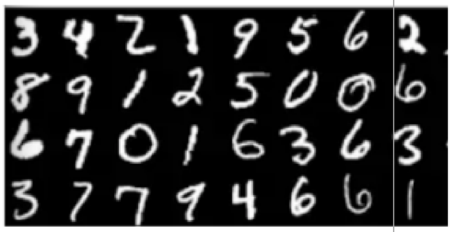
\includegraphics[width=0.6\textwidth]{fig/mnist.png}
\caption{Sample Input Images from MNIST dataset.}
\label{fig1}
\end{figure}

Figure~\ref{fig1}에서 볼 수 있듯이 MNIST 데이터 셋의 입력은 28 x 28 크기의 숫자 이미지이며 이를 벡터화 하여 여러 Layer를 거쳐 마지막에 output layer에 10개의 숫자 중 나타날 확률을 학습하게 된다. 행렬과 벡터 곱셈이 매우 크므로 공간이나 시간적 복잡도를 최적화하기 위해서는 Tiling method를 사용하였으며 이 방법을 CNN 모델의 행렬 곱셈에서도 사용하게 된다. 행렬과 벡터 또는 행렬과 행렬을 일정한 크기로 나누어 가속기를 통해 쓰레드를 나누어 빠른 연산 속도를 가능하게 한다~\cite{lab9, crockett2014zynq, deng2012mnist}.\\

이번 프로젝트에서는 다음과 같이 3가지 Optimization을 이용해서 행렬 곱셈을 가속을 시킬 수 있다.
\begin{enumerate}
    \item DMA (Direct Memory Access)는 CPU와 독립적으로 Main Memory에 접근할 수 있게 해주는 기능이다. Software 단에서 행렬 곱셈에 필요한 데이터를 CDMA 모듈을 통해 효율적으로 전송함에 따라 연산에서 데이터 전송에 걸리는 시간을 줄일 수 있을 것이다.
    \item Quantization (양자화)는 넓은 범위에 분포되어 있는 데이터를 제한된 유한한 범위로 혹은 제한된 자료형으로 매핑하는 과정을 의미한다. 이렇게 함으로써 Quantized 데이터를 연산하는 속도 및 저장공간을 최소화할 수 있을 것이다. 하지만 데이터를 축약하는 과정인 만큼 그만큼 정확도 손실이 발생한다.
    \item Zero-skipping은 행렬 곱셈에 있어 불필요한 Zero 값들을 저장하지 않을 뿐 아니라 곱셈하는 과정에서도 건너뛰는 기능을 말한다. 곱셈 행렬의 크기가 클수록 Nonzero entry 개수가 적을수록 높은 성능을 보일 것이다.
\end{enumerate} 

\section{Implementation}
\label{sec:impl}
Optimized 버전을 모두 포함하여 기본적으로 프로젝트에서 구현해야 하는 공통사항은 다음과 같다.
\begin{enumerate}
    \item \textit{Verilog Matrix-Matrix Multiplication Module}\\
    Lab 6의 PE controller를 변형시켜 Vector-Vector Multiplication Module을 만들고 같은 방식으로 Matrix-Vector Multiplication Module을 구현할 수 있다.
    \item \textit{C Matrix-Matrix Multiplication \& MNIST Classification Module}\\
    위에서 구현한 FPGA 가속기를 사용하거나 CPU를 이용하여 연산할 지에 따라 MNIST Classification을 수행하는 SW 차원의 모듈을 구현해야 한다. 
    \item \textit{Simulation \& Board Implementation} \\
    만들어진 Verilog 모듈을 보드에 올려서 실행하기 전에 Testbench를 만들어 시뮬레이션을 하고 모듈 간의 연결 작업을 시켜준다.
\end{enumerate}

\begin{figure}[htb!]
	\centering
	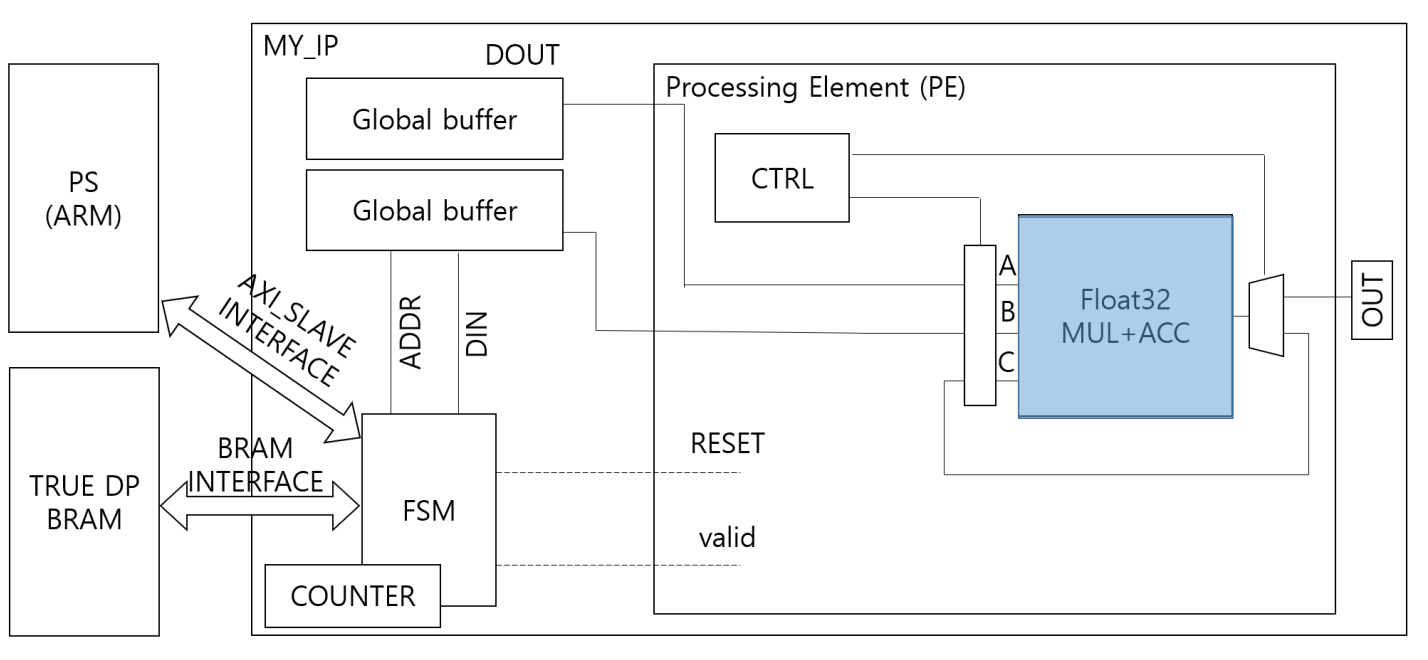
\includegraphics[width=1\textwidth]{fig/overview.png}
\caption{System Overview of the Final Project.}
\label{fig2}
\end{figure}

\newpage
Section~\ref{sec:intro}에서 설명한 Optimization 기능 3개 중 2가지 구현을 하기로 결정하였다. 프로젝트 별로 진행되는 설명의 대략적인 개요는 아래와 같다.

\begin{itemize}
    \item V0
        \begin{itemize}
            \item Verilog: Optimization에서 공통적으로 사용되는 MM-multiplication 모듈 및 테스트벤치에 대한 설명과 함께 AXI에 맞게 BRAM을 연결한 My\_IP 구현을 설명한다.
            \item Software: BRAM과 MM-multiplication을 연결하여 만든 FPGA 모듈을 소프트웨어 내에서 호출하여 연산 가속기를 구현한 내용이 진행된다.
        \end{itemize}
    \item Optimization: DMA
        \begin{itemize}
            \item Verilog: 기본적으로 Verilog 모듈은 V0와 거의 같으므로 중복되는 내용을 제외한 Block design에 있어 달라지는 부분에 초점을 두어 설명한다. 
            \item Software: Verilog에서 크게 달라지는 것이 없는 것에 비해 C 코드에서는 CPU를 거치지 않고 데이터 전송을 원활하게 하기 위한 데이터 복사 구현에 중심을 둔다.
        \end{itemize}
    \item Optimization: Quantization
        \begin{itemize}
            \item Verilog: V0에서 행렬 곱셈을 하고 있던 실수값들을 int로 Quantized한 데이터에 대해 곱셈을 수행하기 위해서 int로 변환된 행렬 곱셈 가속기가 필요하다. 이에 V0에서 달라진 구현과 테스트벤치에 대한 설명이 이어진다.
            \item Software: Quantization에서 가장 중심이 되는 Logic 구현이 이뤄진다. 실수 행렬을 어떻게 int로 매핑하는지 그리고 다시 실수화 시키는지에 대한 아이디어를 중심으로 기술한다.
        \end{itemize}
\end{itemize}

\subsection{V0}

\subsubsection{Verilog}
Software 코드에서 Block 단위로 쪼개어 보내는 단위인 8*8 행렬끼리의 곱셈을 구현한 MM-multiplication 모듈에 대해 코드와 함께 설명이 진행된다.

\subsubsection*{Module \texttt{mm\_multiplier.v}}
\label{sec:mm_mul}
\begin{lstlisting}[style={verilog-style}]
`timescale 1ns / 1ps

module mm_multiplier #(
    parameter L_RAM_SIZE   = 3,
    parameter BITWIDTH     = 32
)(
    input                   start,
    input                   reset,
    input                   clk,
    input  [BITWIDTH-1:0]   rddata,
    output [BITWIDTH-1:0]   wrdata,
    output [2*L_RAM_SIZE:0] addr,
    output                  we,
    output                  done
);
    localparam S_IDLE       = 3'b000;
    localparam S_LD_1       = 3'b010;
    localparam S_LD_2       = 3'b011;
    localparam S_CC_1       = 3'b100;
    localparam S_CC_2       = 3'b101;
    localparam S_HV_1       = 3'b110;
    localparam S_HV_2       = 3'b111;
    localparam S_DONE       = 3'b001;
    
    localparam DONE_LATENCY = 5;
    localparam MAT_SIZE     = 2**(L_RAM_SIZE*2);
    localparam VEC_SIZE     = 2**(L_RAM_SIZE);
    localparam ZERO         = {BITWIDTH{1'b0}};
    
    reg [2*L_RAM_SIZE:0]    cnt_load, cnt_harv;
    reg [L_RAM_SIZE:0]      cnt_calc;
    reg [2:0]               cnt_done;
    reg [2:0]               present_state, next_state;
    reg                     rst_cnt_load, rst_cnt_calc, rst_cnt_harv, rst_cnt_done;
    reg [BITWIDTH-1:0]      gb[0:MAT_SIZE/2*3-1];
    
    wire [BITWIDTH-1:0]     dout[0:MAT_SIZE/2-1];
    wire [MAT_SIZE/2-1:0]   dvalid;
    wire                    valid;
    
    always @(posedge clk or posedge reset)
        if (reset)          present_state <= S_IDLE; 
        else                present_state <= next_state;
    always @(posedge clk or posedge rst_cnt_load) 
        if (rst_cnt_load)   cnt_load <= 0; 
        else                cnt_load <= cnt_load + 1;
    always @(posedge dvalid or posedge rst_cnt_calc) 
        if (rst_cnt_calc)   cnt_calc <= 0;
        else if (dvalid)    cnt_calc <= cnt_calc + 1;
        else                cnt_calc <= cnt_calc;
    always @(posedge clk or posedge rst_cnt_harv) 
        if (rst_cnt_harv)   cnt_harv <= 0; 
        else                cnt_harv <= cnt_harv + 1;
    always @(posedge clk or posedge rst_cnt_done) 
        if (rst_cnt_done)   cnt_done <= 0; 
        else                cnt_done <= cnt_done + 1;
    
    always @(*)
        case (present_state)
            S_IDLE: if (start)                          next_state = S_LD_1; else next_state = present_state;
            S_LD_1: if (cnt_load == MAT_SIZE/2*3-1)     next_state = S_CC_1; else next_state = present_state;
            S_CC_1: if (cnt_calc == VEC_SIZE)           next_state = S_HV_1; else next_state = present_state;
            S_HV_1: if (cnt_harv == MAT_SIZE/2-1)       next_state = S_LD_2; else next_state = present_state;
            S_LD_2: if (cnt_load == MAT_SIZE/2-1)       next_state = S_CC_2; else next_state = present_state;
            S_CC_2: if (cnt_calc == VEC_SIZE)           next_state = S_HV_2; else next_state = present_state;
            S_HV_2: if (cnt_harv == MAT_SIZE/2-1)       next_state = S_DONE; else next_state = present_state;
            S_DONE: if (cnt_done == DONE_LATENCY-1)     next_state = S_IDLE; else next_state = present_state;
            default: next_state = present_state;
        endcase
    
    always @(posedge clk)
        case (present_state)
            S_LD_1, S_LD_2: {rst_cnt_load, rst_cnt_calc, rst_cnt_harv, rst_cnt_done} <= 4'b0111;
            S_CC_1, S_CC_2: {rst_cnt_load, rst_cnt_calc, rst_cnt_harv, rst_cnt_done} <= 4'b1011;
            S_HV_1, S_HV_2: {rst_cnt_load, rst_cnt_calc, rst_cnt_harv, rst_cnt_done} <= 4'b1101;
            S_DONE:         {rst_cnt_load, rst_cnt_calc, rst_cnt_harv, rst_cnt_done} <= 4'b1110;
            default:        {rst_cnt_load, rst_cnt_calc, rst_cnt_harv, rst_cnt_done} <= 4'b1111;
        endcase
        
    integer j;
    always @(posedge clk) begin
        for (j = 0; j < MAT_SIZE/2*3; j = j+1)                      gb[j]        = gb[j];
        case (present_state)
            S_IDLE: for (j = 0; j < MAT_SIZE/2*3; j = j+1)          gb[j]        = 0;
            S_LD_1, S_LD_2:                                         gb[cnt_load] = rddata;
            S_HV_1, S_HV_2: for (j = 0; j < MAT_SIZE/2; j = j+1)    gb[j]        = dvalid ? dout[j] : gb[j];
        endcase
    end
    
    assign addr   = (present_state == S_LD_1 ? (cnt_load < MAT_SIZE/2 ? cnt_load : cnt_load+MAT_SIZE/2) : 
                    (present_state == S_LD_2 ? cnt_load+MAT_SIZE/2 :
                    (present_state == S_HV_1 ? cnt_harv : 
                    (present_state == S_HV_2 ? cnt_harv+MAT_SIZE/2 : 0))));
    assign wrdata = (present_state == S_HV_1 || present_state == S_HV_2) ? gb[cnt_harv] : 0;
    assign we     = (present_state == S_HV_1 || present_state == S_HV_2);
    assign done   = (present_state == S_DONE);
    assign valid  = (present_state == S_CC_1 || present_state == S_CC_2) ? ~dvalid : 0;
    
    genvar i;
    generate for (i = 0; i < MAT_SIZE/2; i = i+1) begin: MATRIX
        wire [BITWIDTH-1:0] ain = gb[(i/VEC_SIZE)*VEC_SIZE + cnt_calc];
        wire [BITWIDTH-1:0] bin = gb[cnt_calc*VEC_SIZE + (i%VEC_SIZE) + MAT_SIZE/2];
        my_pe #(L_RAM_SIZE, BITWIDTH) MY_PE(
            .aclk(clk),
            .aresetn(~(reset || present_state == S_LD_2 || present_state == S_DONE)),
            .ain(valid ? ain : 0),
            .bin(valid ? bin : 0),
            .valid(valid),
            .dvalid(dvalid[i]),
            .dout(dout[i])
        );
    end endgenerate
endmodule
\end{lstlisting}

mm\_multiplier는 PE Controller에서 확장된 구조를 가지고, 따라서 동일한 FSM의 논리를 통해 구현하였다. PE Controller에서 확장된 점은, Matrix-Matrix multiply를 위한 Matrix를 Global buffer에 저장한 뒤, PE에 전달, 이후 연산을 진행한다는 것이다.\\\\
mm\_multiplier는 IDLE, LOAD\_1,2, CALC\_1,2, HARV\_1,2, DONE의 7가지 state를 가진다. IDLE은 대기 상태를 의미하며, 이 때 \texttt{start} 신호가 입력되면 LOAD\_1 state로 전이된다. 이 상태에서는 \texttt{rdaddr} 주소를 Testbench에 전달하여 \texttt{rddata} 값을 하나씩 입력받아 Global buffer에 저장한다.

\begin{itemize*}
\item 상기된 코드 중 3-39 라인은 MM multiplier의 변수 선언에 관한 내용이다.
\begin{itemize*}
\item \texttt{parameter}에 포함된 (1) \texttt{L\_RAM\_SIZE}는 입력되는 Matrix의 크기를 표현하는 상수이고, (2) \texttt{BITWIDTH}는 연산을 하기 위한 실수 자료형의 크기를 나타낸다.
\item FSM과 관련된 변수는 현재 상태와 앞으로 업데이트해야하는 상태 변수 \texttt{present\_state}와 \texttt{next\_state}가 있고 그 외에 Counter가 있다. 상태를 나타내는 상수는 총 5가지로 $0 \sim 7$의 값을 \texttt{S\_IDLE}, \texttt{S\_LD\_1}(=\texttt{LOAD}), \texttt{S\_LD\_2}, \texttt{S\_CC\_1}(=\texttt{CALC}) \texttt{S\_CC\_2}, \texttt{S\_HV\_1}(=\texttt{HARV}),  \texttt{S\_HV\_2}와 \texttt{S\_DONE}에 해당하도록 설정하였다.
\item 내장 모듈인 MY\_PE의 입출력 변수 \texttt{ain}, \texttt{bin}, \texttt{valid}, \texttt{dout}, \texttt{dvalid}, \texttt{valid}를 함께 선언하고 지정시켜주어야 한다.
\end{itemize*}

\item 41-56 라인과 58-69 라인은 강의시간에 배운 FSM의 format을
그대로 차용하여 구현하였다. 초기 상태를 \texttt{reset} 신호와 함께 IDLE 상태로 초기화 한다. 현재 상태에서 어떤 조건이 중족되었을 때 다음 상태를 지정해주는 논리를 구현해준다.

\item 71-97라인은 각 상태에 위치했을 때 어떤 Counter를 활성화 시킬지 지정해주는 부분이다. 74-77라인에서는 현재 상태가 LOAD에 이르렀을 때 테스트벤치로 \texttt{rdaddr}을 전달해주고 해당하는 실수형 자료 \texttt{rddata}를 받아와 Global buffer에 저장한다.

\item 99-112라인은 \texttt{generate}문에서 PE 모듈 인스턴스를 생성하여, Matrix-Matrix multiply를 수행한다.
\end{itemize*}

\begin{figure}[ht]
	\centering
	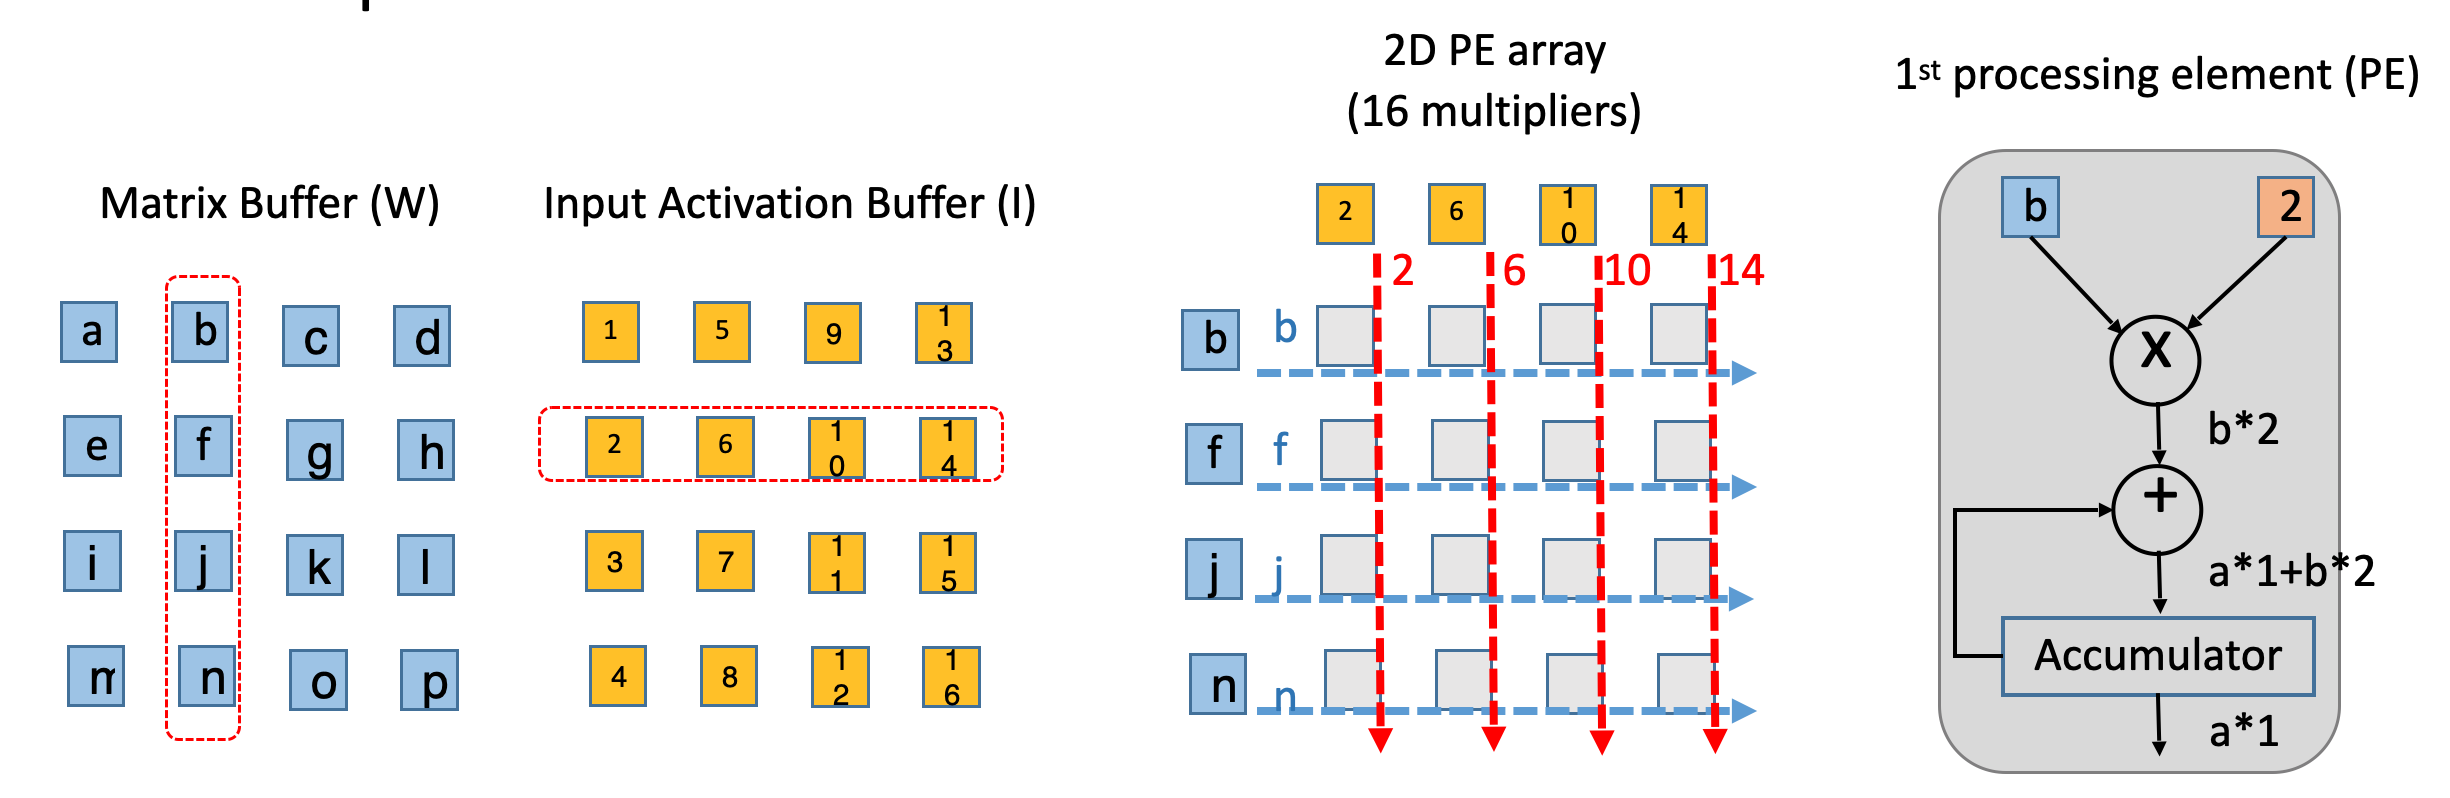
\includegraphics[width=0.8\textwidth]{fig/broadcast_mm.png}
\caption{Broadcast \& PE computation process}
\label{fig3}
\end{figure}
모든 LOAD 과정이 끝나면, Figure~\ref{fig3}에서의 방법과 같은 방식으로, CALC 단계에서 FP IP\cite{FP_MAC} catalog를 수행하게 된다. Global buffer에 저장된 VECTOR\_SIZE(=64)크기의 열벡터와 행벡터를 추출하여 Multiply-Accumulator를 이용해 내적 값을 구하게 된다. Multiply-Accumulator연산이 모두 끝난 후, \texttt{cnt\_calc}값은 1증가하고, 다음 사이클을 진행한다. 모든 MM연산을 마치면, state는 HARV로 넘어가고, 최종 결과 Matrix와 wrdata를 통해 결과값을 저장한다. 이후, state는 DONE으로 넘어가게 되고 5(Latency)사이클 동안 \texttt{done} signal을 출력한다. 이후에는 다시 state를 IDLE 상태로 돌려 놓고 \texttt{start} 신호를 기다린다.\\

위의 설명은 V0\_mid에서 구현한 방식이다. 하지만,implementation \& generate bitstream을 하는 과정에서는 위의 방법을 naive하게 적용하기에는 무리가 있었다. 상기된 모듈에서는 $64\times64$ matrix multiplication을 수행해야 한다. 하지만, 두 행렬 전체를  load하여 곱하는 방법으로는 register가 부족한 현상이 발생한다. 따라서,  weight matrix 전체 행 중 절반만 load하여 \texttt{LD\_1} state에서 input activation matrix와 곱하고, 나머지 절반을 load하여 \texttt{LD\_2} state에서 activation matrix와 곱해주었다. 나머지 state에서 동작방식은 V0\_mid와 동일하다.\\\\
이러한 방식을 적용하였을 때, \texttt{LOAD}(=\texttt{LD\_1}, \texttt{LD\_2}), \texttt{CALC}(=\texttt{CC\_1}, \texttt{CC\_2}), \texttt{HARV}(=\texttt{HV\_1}, \texttt{HV\_2}) state에서 모듈의 동작방식은  다음과 같다.
\begin{itemize*}
    \item 35라인은 gb(global buffer)을 나타낸다. \texttt{LOAD} state에서 load된 값들이 저장된다. 또한, \texttt{CALC} state에서 계산이 끝나면, 결과값을 gb에 넣고, \texttt{HARV} state에서 global buffer의 값을 읽어 최종 결과값을 출력한다.
    \item 37라인은 dout, 즉, output을 나타낸다. \texttt{CALC} state에서 계산된 결과가 저장된다.
    \item 99-111라인은 weight matrix를 나누고, my\_pe모듈에 input을 할당해준다. \texttt{ain}, \texttt{bin}은 101, 102라인에서 선언되는데, 절반으로 나눠진 weight matrix와 input activation matrix전체를 inner product를 통해 곱해줄 수 있도록 index를 할당하였다.
\end{itemize*}


\subsubsection*{Module \texttt{tb\_mm\_multiplier.v}}
\begin{lstlisting}[style={verilog-style}]
`timescale 1ns / 1ps

module tb_mm_multiplier #(
    parameter L_RAM_SIZE = 3,
    parameter BITWIDTH = 32,
    parameter INFILE = "global_buffer_in.txt",
    parameter OUTFILE = "global_buffer_out.txt"
)();
    localparam MATRIX_SIZE = 2**(L_RAM_SIZE*2);
    localparam VECTOR_SIZE = 2**(L_RAM_SIZE);
    reg [BITWIDTH-1:0] rdgb[0:MATRIX_SIZE*2-1];
    reg [BITWIDTH-1:0] wrgb[0:MATRIX_SIZE-1];
    wire [BITWIDTH-1:0] rddata;
    wire [BITWIDTH-1:0] wrdata;
    wire [2*L_RAM_SIZE:0] addr;
    wire done, we;
    
    reg start, clk, reset;
    integer i;
//    initial begin
//        for(i = 0; i < MATRIX_SIZE; i = i+1) begin
//            rdgb[i]               = $urandom_range(2**30, 2**30+2**24);
//            rdgb[MATRIX_SIZE + i] = $urandom_range(2**30, 2**30+2**24);
//        end
//        $writememh(INFILE, rdgb);
//    end
    assign rddata = start ? rdgb[addr] : 0;
    initial begin
        $readmemh(INFILE, rdgb);
        for(i = 0; i < MATRIX_SIZE; i = i+1) wrgb[i] <= 0;
        clk <= 0;
        start <= 0; reset <= 1; 
        #10 start <= 1; reset <= 0;
    end
    always @(*)
        if (we) wrgb[addr] = wrdata;
    always @(posedge done) begin
        $writememh(OUTFILE, wrgb);
    end
    
    always #1 clk = ~clk;
    mm_multiplier #(L_RAM_SIZE, BITWIDTH) MM_MULTIPLIER(
        .start(start),
        .reset(reset),
        .clk(clk),
        .addr(addr),
        .rddata(rddata),
        .wrdata(wrdata),
        .we(we),
        .done(done)
    );
endmodule
\end{lstlisting}
tb\_mm\_multiplie 모듈에서는 mm\_multiplier모듈의 parameter값들을 tb\_mm\_multiplier 모듈의 4-7라인에서 초기화하고, 9-19라인에서 in-put 및 output값들을 초기화시킨다. Matrix 2개의 값들은 glboal\_buffer\_in.txt에 저장한다. 해당 텍스트 파일에 저장된 값을 읽어들여, glboal\_buffer\_out.txt로 결과값을 출력시킨다. 일단 input파일에 저장되면, 해당 부분을 주석처리하여 동일한 input value를 사용함으로서, seed를 사용하여 실험하는 것과 비슷한 효과를 낼 수 있다. \\

Appendix~\ref{sec:float}의 표는 테스트벤치에서 생성된 실수 행렬을 저장한 입력 파일에서 행렬 A와 B를 읽어와 모듈 \texttt{mm\_mul}을 통해 연산한 행렬 C를 연산한 결과이다. 표의 상단 부분은 16진수 형태의 single precision floating point 자료형이고 하단부는 Python hex-to-float decoder를 통해 실수 형태로 변환한 결과이다. 행렬 곱셈연산이 제대로 수행됨을 확인할 수 있다.

\subsubsection*{Module \texttt{myip\_v1\_0\_S00\_AXI.v}}
\label{sec:s00}
아래는 해당 모듈의 block design figure와 verliog 코드이다.
\begin{figure}[ht]
	\centering
	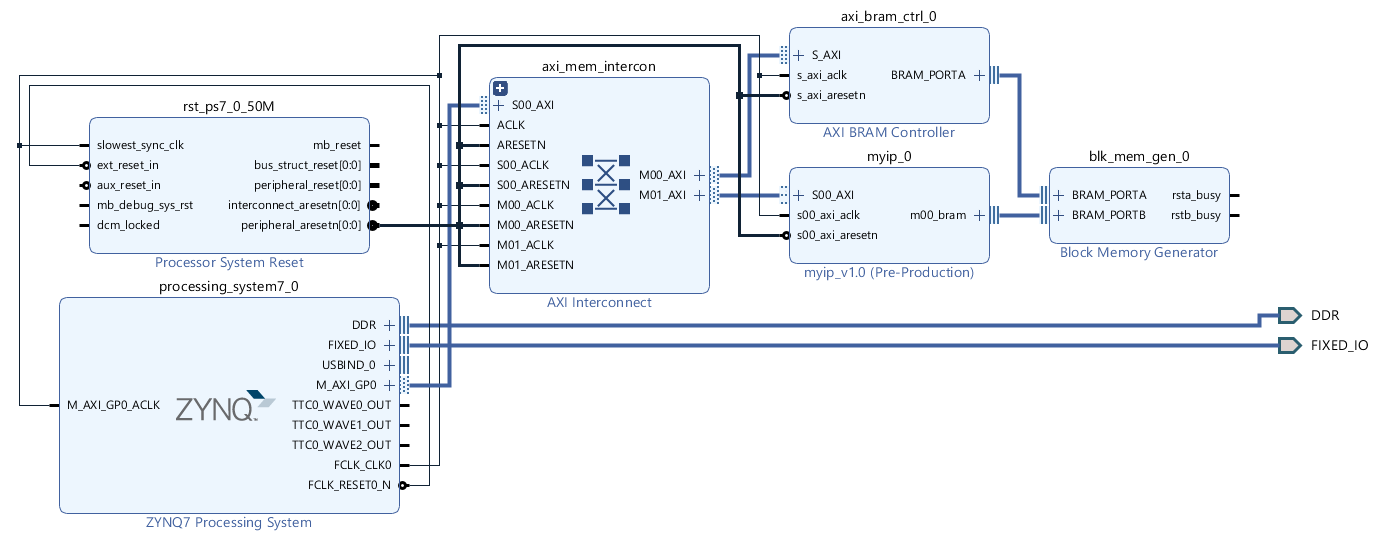
\includegraphics[width=1.0\textwidth]{fig/V0/design.png}
\caption{Block Design for V0}
\label{design_v0}
\end{figure}

\begin{lstlisting}[style={verilog-style}]
localparam L_RAM_SIZE = 3;
localparam BITWIDTH = 32;

wire start, done, we;
wire [2*L_RAM_SIZE:0] addr;
clk_wiz_0 u_clk_180 (.clk_out1(BRAM_CLK), .clk_in1(S_AXI_ACLK));

assign start = (slv_reg0 == 32'h5555);
assign run_complete = (done);

assign BRAM_EN  = 1'b1;
assign BRAM_RST = 1'b0;
assign BRAM_WE  = we ? 4'hF : 4'h0;
assign BRAM_ADDR = {addr, 2'd0};

mm_multiplier #(L_RAM_SIZE, BITWIDTH) MM_MULTIPLIER(
    .start(start),
    .reset(~S_AXI_ARESETN),
    .clk(S_AXI_ACLK),
    .rddata(BRAM_RDDATA),
    .wrdata(BRAM_WRDATA),
    .addr(addr),
    .we(we),
    .done(done)
);
\end{lstlisting}
\texttt{myip\_v1\_0\_S00\_AXI.v}는 MM multiplication을 위한 IP를 customizing 할 때, wire를 연결하고, software 코드에서 my\_ip를 접근하기 위한 register의 주소를 할당해주는 역할을 한다. 기존 texttt{myip\_v1\_0\_S00\_AXI.v}파일에서 user logic을 추가하는 부분만 수정하여 Custom IP를 생성하였다.\\\\
아래는 상기된 코드에 대한 설명이다.
\begin{itemize*}
    \item 1-4, 11-14라인은 MM multiplier 모듈에서 필요한 parameter, \texttt{BRAM}에 접근하기 위한 wire를 할당해준다.
    \item 6라인은 \texttt{clk\_wiz\_0}모듈을 사용하는데, 이는 BRAM과 AXI clock sync를 맞춰주는 역할을 한다.
    \item 16-25라인은 우리가 구현한 \texttt{mm\_multiplier}모듈의 input, output을 할당해준다.
\end{itemize*}

\subsubsection{Software}
과 마찬가지로 Tiling Method으로 축소 대응시켜 계산을 하면 된다. 함수를 사용하기 위해서 중간 중간에 \texttt{data\_M}라는 데이터 중간 저장소를 통해 곱셈에 사용될 2개의 행렬을 fetching 하고 연산된 output vector를 덮어쓰는 과정을 반복하게 된다.

Figure~\ref{fig3}에서 볼 수 있듯이 기본적으로 \texttt{v\_size} 간격으로 작은 Block operation을 수행하지만 행렬의 가로, 세로 크기가 항상 \texttt{v\_size}의 배수가 아니므로 경계부분에서의 예외처리를 위해 Block 사이즈를 나타내는 변수 \texttt{block\_row},  \texttt{block\_col\_1}, \texttt{block\_col\_2}를 도입한다.

\subsubsection*{\texttt{FPGA::largeMM}}
아래의 코드는 fpga\_api.cpp 코드의 일부를 나타낸다.\\
\begin{lstlisting}[style={c-style}]
void FPGA::largeMM(const float* weight_mat, const float* input_mat,
        float* output, int num_input, int num_output, int num_matrix2) {
  float* m1 = this->matrix_M1();
  float* m2 = this->matrix_M2();

  // 0) Initialize output vector		
  for(int i = 0; i < num_output*num_matrix2; ++i)
    output[i] = 0;

  for(int i = 0; i < num_output; i += v_size_) {
    for(int j = 0; j < num_input; j += v_size_) {
      for(int k = 0; k < num_matrix2; k += v_size_) {
      
        // 0) Initialize input vector
        int block_row = min(v_size_, num_output-i);
        int block_col_1 = min(v_size_, num_input-j);
        int block_col_2 = min(v_size_, num_matrix2-k);

        // 1) Assign a m1
        for (int row = 0; row < block_row; row++) {
          for (int col = 0; col < block_col_1; col++)
            m1[row*v_size_ + col] = weight_mat[(i+row)*num_input + (j+col)];
          for (int col = block_col_1; col < v_size_; col++)
            m1[row*v_size_ + col] = 0;
        }
        for (int l = block_row*v_size_; l < m1_size_; l++)
            m1[l] = 0;
        
        // 2) Assign a m2
        for (int row = 0; row < block_col_1; row++) {
          for (int col = 0; col < block_col_2; col++)
            m2[row*v_size_ + col] = input_mat[(j+row)*num_matrix2 + (k+col)];
          for (int col = block_col_2; col < v_size_; col++)
            m2[row*v_size_ + col] = 0;  
        }
        for (int l = block_col_1*v_size_; l < m2_size_; l++)
            m2[l] = 0;
        
        // 3) Call a function `blockMM() to execute Matrix matrix multiplication
        const float* ret = this->blockMM();

        // 4) Accumulate intermediate results
        for(int n = 0; n<block_row; ++n) {
          for(int m = 0; m<block_col_2; ++m) {
            output[(i + n) + (k + m)*num_output] += ret[n*v_size_ + m];
          }
        }
      }
    } 
  }
}
\end{lstlisting}

\begin{itemize*}
\item Block OP를 수행할 부분인 Weight matrix를 \texttt{m1}에 먼저 넣는다 (20-25 라인).
\item 이 행렬의 크기는 \texttt{block\_row} * \texttt{block\_col\_1} 이므로 첫 번째 행렬 부분에 해당하는 \texttt{m1\_size\_} 중 사용하지 않는 부분은 모두 0으로 초기화한다 (26-27 라인).
\begin{itemize*}
\item 그렇지 않다면 전 step에서 사용되었던 벡터 값이 잘못된 연산 결과를 초래할 수 있기 때문이다~\cite{lab2}.
\end{itemize*}
\item 다음으로 Input matrix를 \texttt{m2}에 넣는다 (30-35 라인). 
\item 이 행렬의 크기는 \texttt{block\_col\_2} * \texttt{block\_col\_1} 이므로 두 번째 행렬 부분에 해당하는 \texttt{m2\_size\_} 중 사용하지 않는 부분은 모두 0으로 초기화한다 (36-37 라인).
\item \textit{largeMM} 함수에서 데이터를 parameter로 받아서, custom IP가 실행되는 함수인 block\_MM을 실행한다 (40 라인).
\item Tiling된 결과를 output에 더해서 최종 결과를 얻는다 (43-47 라인).
\end{itemize*}

\subsubsection*{\texttt{FPGA::blockMM}}
\begin{lstlisting}[style={c-style}]
const float* __attribute__((optimize("O0"))) FPGA::blockMM() {
  num_block_call_ += 1;
  // fpga version
  *output_ = 0x5555;
  while(*output_ == 0x5555);
  return data_M;    
}
\end{lstlisting}
위는 실제 FPGA Custom IP가 호출되는 함수이다. 6 번째 줄에서, output포인터에 0x5555를 할당해주는데, 이로서 Custom\_IP에 output이 mapping된다. 왜냐하면 Section~\ref{sec:s00} \texttt{my\_ip\_v1.0\_S00\_AXI.v}에서 확인할 수 있다.

\newpage
\subsection{Optimization: DMA}

\begin{figure}[htb!]
	\centering
	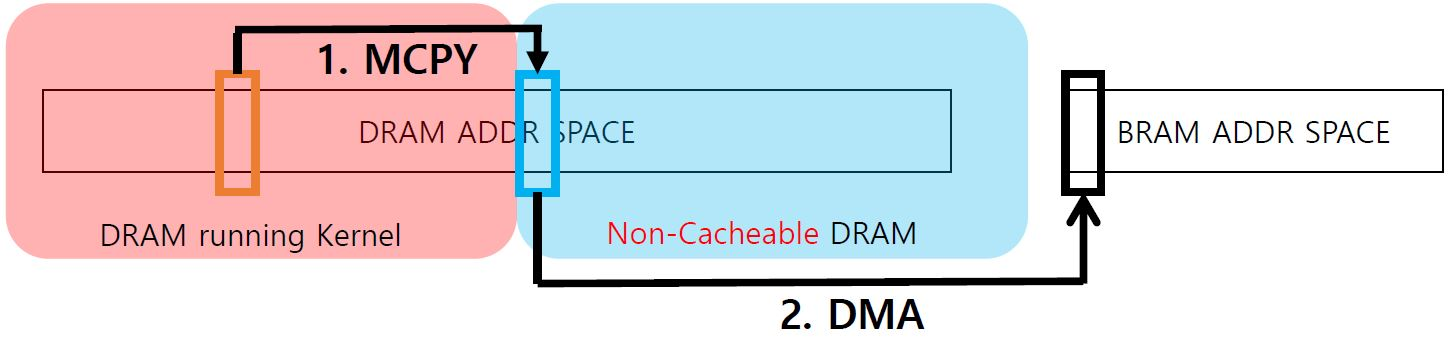
\includegraphics[width=0.8\textwidth]{fig/V1_DMA/overview.jpg}
\caption{Memcopy and DMA Process with BRAM~\cite{lab11}.}
\label{fig:lab11}
\end{figure}

\subsubsection{Verilog}

\begin{figure}[htb!]
	\centering
	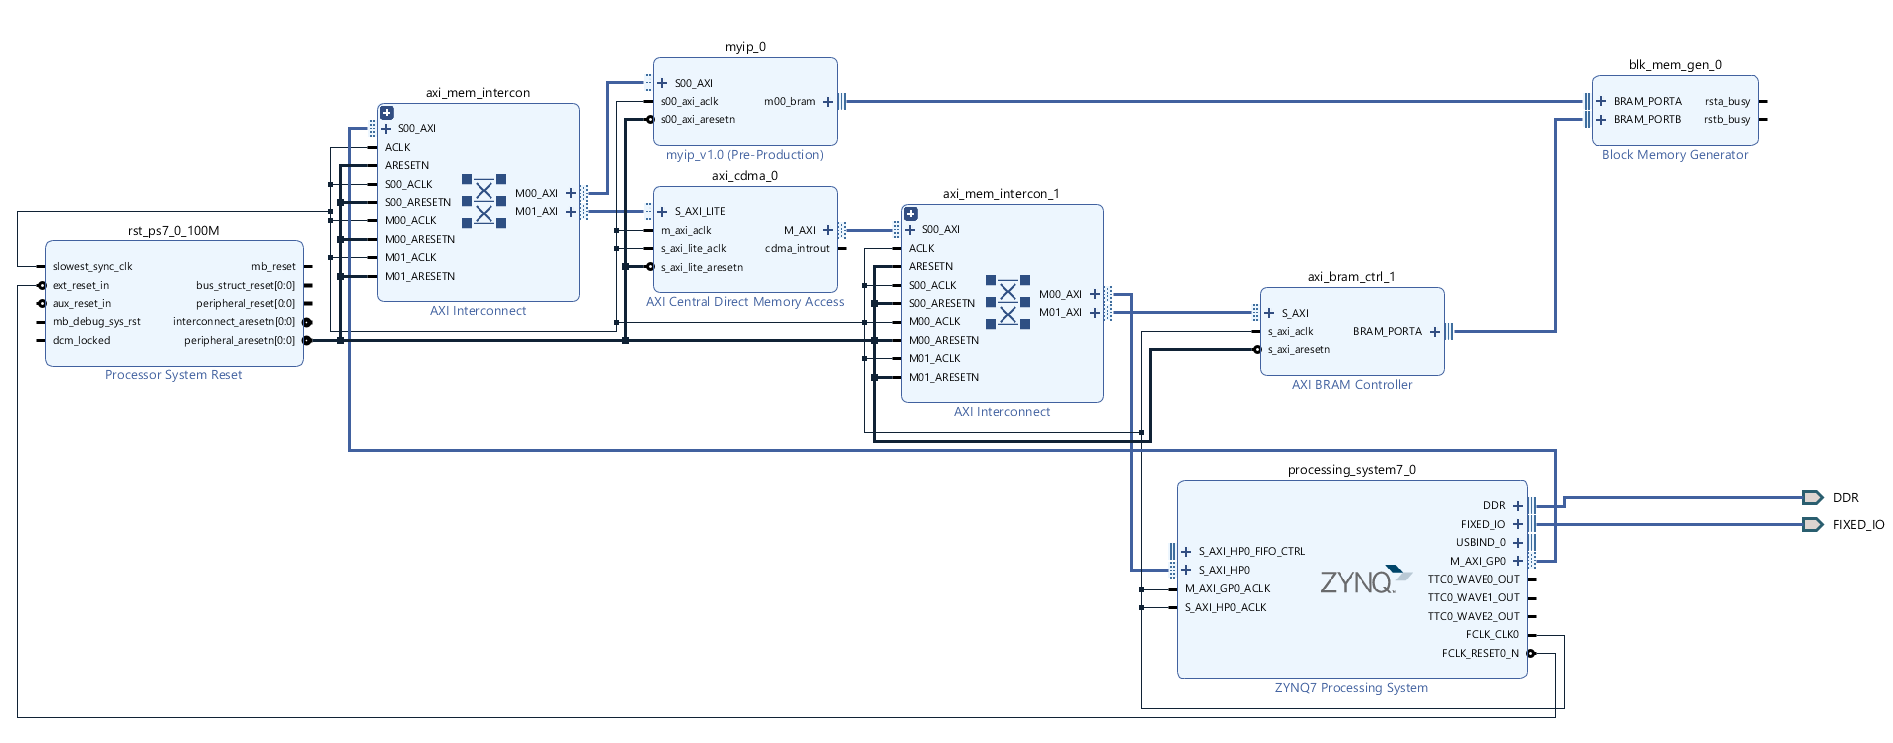
\includegraphics[width=1.0\textwidth]{fig/V1_DMA/design.png}
\caption{Block Design for V1\_DMA}
\label{design_v1_dma}
\end{figure}

Figure~\ref{fig:lab11}에서 처럼 CPU를 거치지 않고 CDMA 모듈을 썼을 때 V0에서 구현한 My\_IP 모듈이 어디에 해당하는 위치에 Place Design 되어야 하는지가 관건이다. CDMA가 있는 \texttt{block\_design\_cmda.tcl}을 실행했을 때 생기는 Block design 중 \textit{axi\_bram\_ctrl\_0}을 수정하면 된다.\\

Figure~\ref{design_v1_dma}에서 볼 수 있듯이 기존의 BRAM 제어 모듈을 지우고 My\_IP 모듈로 대체된 것을 볼 수 있다. 이렇게 bitstream을 생성하여 Zed board에서 부팅을 하면 이제 \textit{axi\_bram\_ctrl\_0}에서 수행하던 역할을 CDMA 모듈을 활용하여 Software에서도 데이터 접근이 가능할 것이다. 이때 참조할 수 있는 주소는 미리 할당된 CDMA address (0x7E200000 - 0x7E20FFFF)이다. (보다 자세한 내용은 Lab 11의 보고서를 참고).

\subsubsection{Software}

\begin{figure}[htb!]
	\centering
	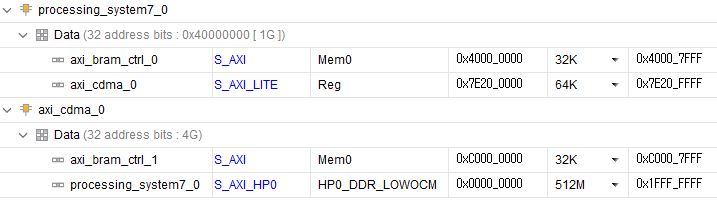
\includegraphics[width=0.7\textwidth]{fig/V1_DMA/address.jpg}
\caption{CDMA Address for V1\_DMA}
\label{address_v1_dma}
\end{figure}

DMA를 사용한 memory load의 속도 개선은 결과적으로 training, inference time의 속도 개선을 의미한다. Software에서 CDMA의 기능을 활용하기 위해서는 다음과 같은 과정으로 진행할 수 있다. \texttt{mmap()} 함수를 통해, bitstream에서 미리 할당된 CDMA address(0x7E200000 - 0x7E20FFFF)를 메모리 (fpga\_dma)에 대응시킨다 (Figure~\ref{address_v1_dma}). CDMA IP에 올바른 input값들 (source addr, dest addr, bytes to transfer)을 할당하고, DMA operation이 종료될 때까지 기다린다~\cite{CDMA}.

\subsubsection*{py\_lib.cpp}
\begin{lstlisting}[style={c-style}]
// ...
void *getCaffeNet(void *network, int m_size, int v_size)
{
  char *net_char = static_cast<char *>(network);
  FPGA *dev = new FPGA(0x7E200000, 0x10000000, 0xC0000000, 0x43C00000, m_size, v_size);
  return new CaffeDNN(std::string(net_char), dev);
}
// ...
void *getTFNet(void *network, int m_size, int v_size) {
  char *net_char = static_cast<char *>(network);
  FPGA *dev = new FPGA(0x7E200000, 0x10000000, 0xC0000000, 0x43C00000, m_size, v_size);
  return new TFDNN(std::string(net_char), dev);
}
// ...
\end{lstlisting}

\subsubsection*{fpga\_api.cpp}
\begin{lstlisting}[style={c-style}]
// ...
FPGA::FPGA(off_t fpga_dma_addr, off_t _noncache_addr, off_t _bram_addr, off_t output_addr, int m_size, int v_size)
{
  m_size_       = m_size;
  v_size_       = v_size;
  m1_size_      = v_size * v_size;
  data_size_    = (m_size_+1)*v_size_;
  data_size_M   = (2*v_size_)*v_size_*sizeof(float);
  data_         = new float[data_size_];	

  fd_ = open("/dev/mem", O_RDWR);
  bram_addr     = (float *) _bram_addr;
  noncache_addr = (float *) _noncache_addr;
  data_noncache = static_cast<float*>(mmap(NULL, data_size_M, 
                                    PROT_READ|PROT_WRITE, MAP_SHARED, fd_, _noncache_addr));
  fpga_dma      = static_cast<unsigned int *>(mmap(NULL, sizeof(unsigned int)*16, 
                                    PROT_READ|PROT_WRITE, MAP_SHARED, fd_, fpga_dma_addr));
  data_M        = new float[data_size_M];	

  output_       = static_cast<unsigned int*>(mmap(NULL, sizeof(unsigned int), 
                                    PROT_READ|PROT_WRITE, MAP_SHARED,fd_, output_addr));
  output_MV     = new unsigned int[m_size_];
  // output_M = static_cast<unsigned int*>(NULL);

  num_block_call_ = 0;
}

void __attribute__((optimize("O0"))) FPGA::transfer(const float *src, const float *dst, const unsigned int size) {
  *(fpga_dma + 6) = (unsigned int) src;
  *(fpga_dma + 8) = (unsigned int) dst;
  *(fpga_dma + 10) = size;
  while ((*(fpga_dma + 1) & 0x00000002) == 0);
}

const float* __attribute__((optimize("O0"))) FPGA::blockMM()
{
  num_block_call_ += 1;

  memcpy(data_noncache, data_M, data_size_M);
  transfer(noncache_addr, bram_addr, data_size_M);

  *output_ = 0x5555;
  while(*output_ == 0x5555);
  
  transfer(bram_addr, noncache_addr, data_size_M/2);
  memcpy(data_M, data_noncache, data_size_M/2); 

  return data_M;    
}
// ...
\end{lstlisting}

기존에 FPGA 생성자와는 다르게 Figure~\ref{fig:lab11}에서 여러 주소가 필요한 만큼 초기값으로 주어야하는 주소값들이 많다. \texttt{py\_lib.cpp} 소스코드 5, 11 line에서 \texttt{0x7E200000, 0x10000000, 0xC0000000, 0x43C00000} 값이 전달되는 것을 확인할 수 있다. 이는 각각 (1) CDMA, (2) Non-cacheable memory, (3) BRAM, (4) FPGA magic 주소를 의미한다. 아래의 FPGA 생성자를 보면 쉬운 이해가 가능할 것이다. \\

CDMA 모듈을 활용하는 부분은 Lab 11과 동일하다. \texttt{FPGA::transfer}에서 (1) \texttt{fpga\_dma+6}은 24 (=\texttt{0x18})의 offset을 가지고 SA register, (2) \texttt{fpga\_dma+8}은 32 (=\texttt{0x20})의 offset을 가지고 DA register, (3) \texttt{fpga\_dma+10}은 40 (=\texttt{0x28})의 offset을 가지고 BTT (Bytes To Transfer) register를 가리킴을 확인할 수 있다. 이 같은 방식으로 CDMA 모듈을 활용해 데이터 전송에 걸리는 시간을 최소화할 수 있다~\cite{CDMA}. \\

\texttt{FPGA::blockMM} 함수에서는 V0에서처럼 Magic code (=\texttt{0x5555})를 넣어주어 행렬 연산의 결과값을 가져올 수 있다. 전후에 Figure~\ref{fig:lab11}의 (1)과 (2)의 과정을 통해 BRAM에 행렬 값들을 미리 넣어주고 추출하는 과정이 필요하다 (39-46 라인).

\newpage
\subsection{Optimization: Quantization}
\begin{figure}[htb!]
	\centering
	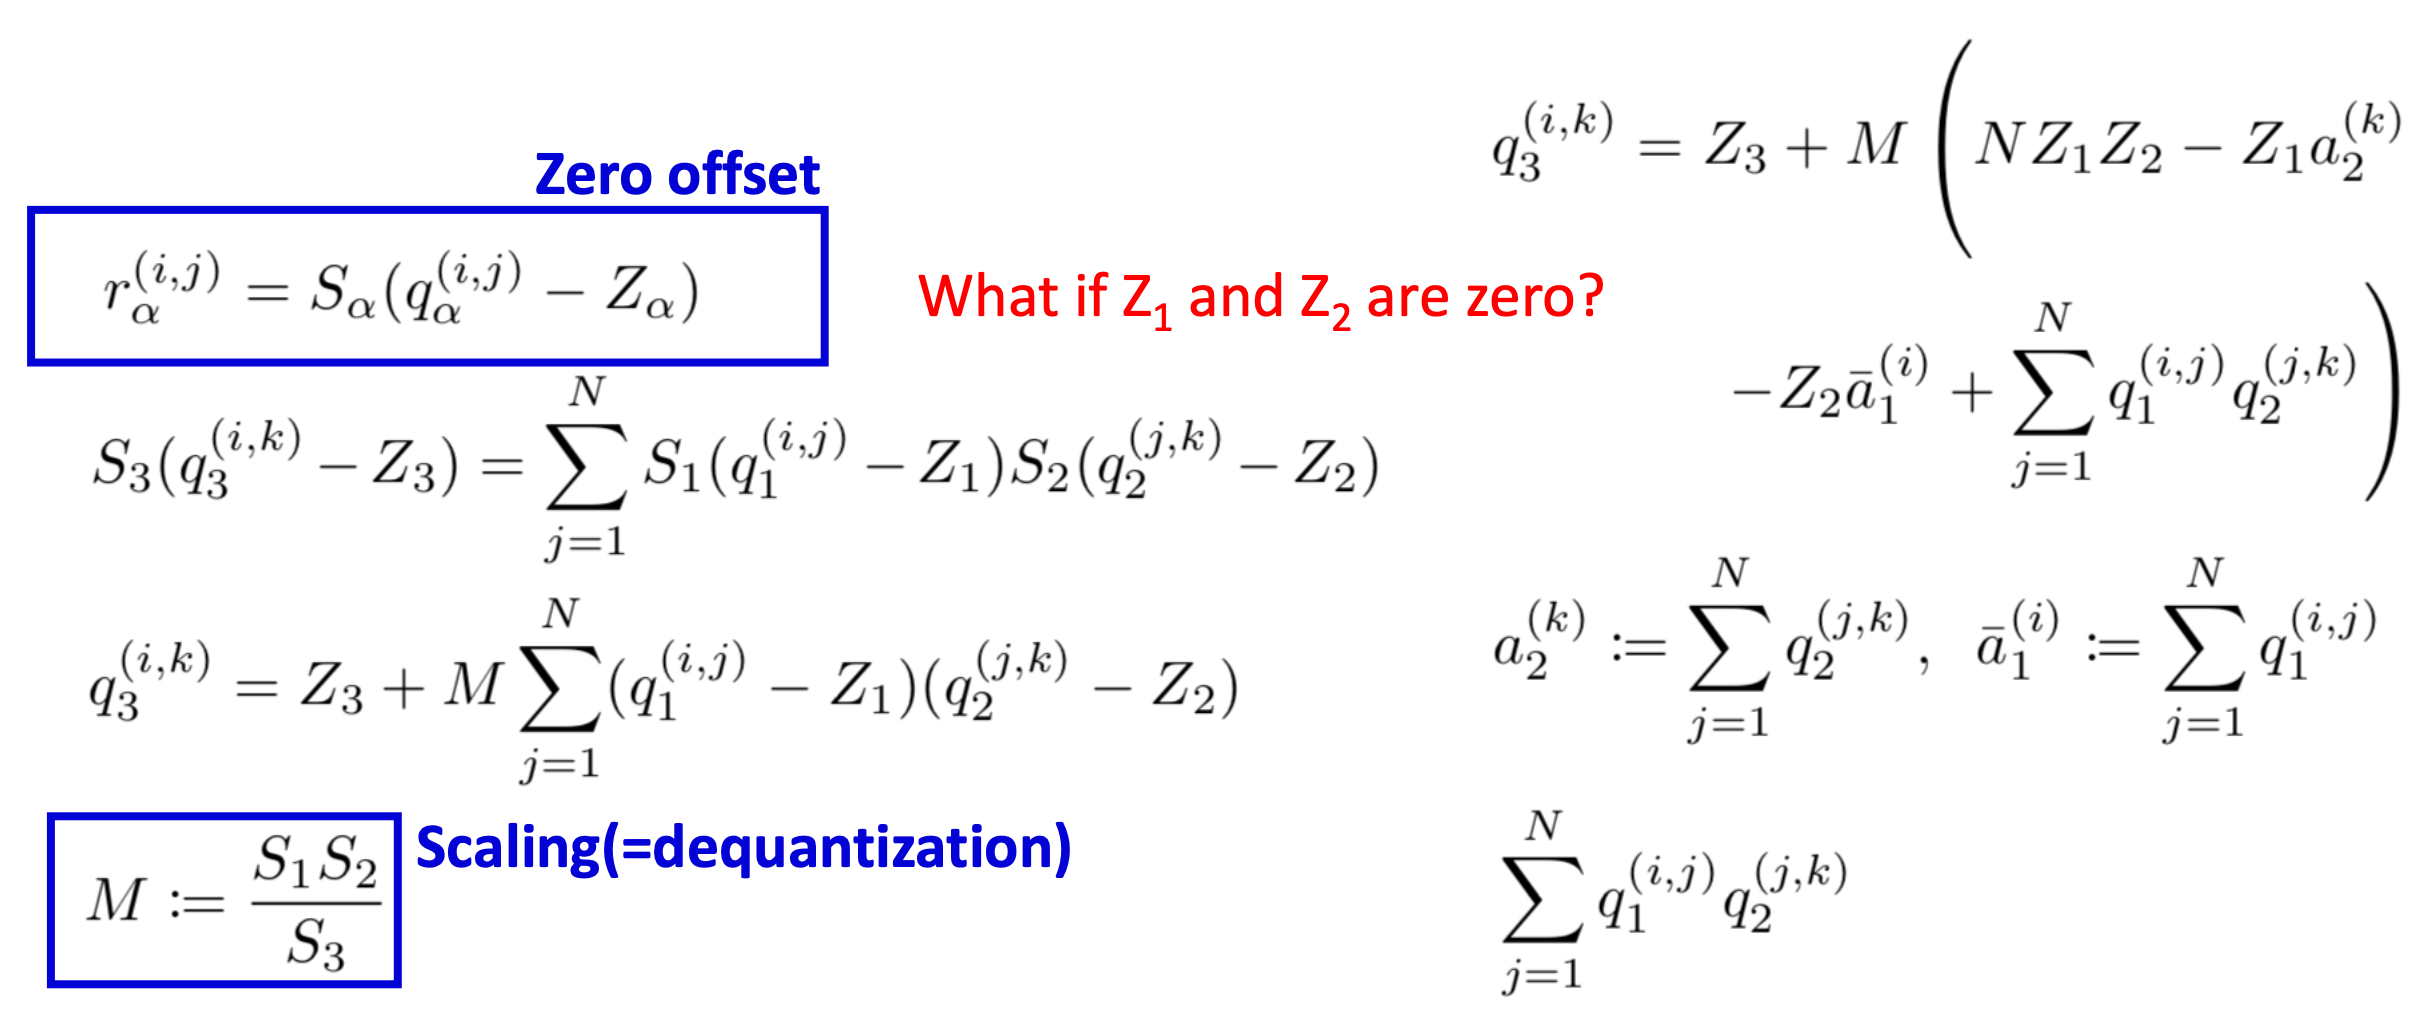
\includegraphics[width=1.0\textwidth]{fig/V1_Quantization/mm_mul_quant.png}
\caption{Matrix Matrix multiplication using quantization}
\label{mm_mul_quant}
\end{figure}

\begin{equation*}
    q_{1(i,j)} = r_{1(i,j)}/S_1 + Z_1, \quad
    q_{2(i,j)} = r_{2(i,j)}/S_2 + Z_2
\end{equation*}
\begin{align*}
    r_{3(i,j)} 
    &= \sum_k r_{1(i,k)} r_{2(k,j)} \\
    &= \sum_k S_1(q_{1(i,k)} - Z_1) \times S_2(q_{2(k,j)} - Z_2) \\
    &= S_1 S_2\left(\sum_k q_{1(i,k)} q_{2(k,j)} - \left( Z_1 \sum_k q_{2(i,k)} + Z_2 \sum_k q_{1(i,k)} - N Z_1 Z_2\right) \right) \\
    &= S_1 S_2\left(\sum_k q_{1(i,k)} q_{2(k,j)} - \left( Z_1 a_2 + Z_2 a_1 - N Z_1 Z_2\right) \right) \\
    &= S_3 (q_3 - Z_3)
\end{align*}

\subsubsection{Verilog}
Quantization의 Integer Matrix Multiplication을 위한 \texttt{Integer MAC}모듈은 IP catalog multiply-adder\cite{Multiply_Addder} 대신에, 직접 작성하여 기존 \texttt{Floating Point MAC}에서 16사이클이 이후에 dvalid가 high가 되는데, Integer MAC에서는 1사이클만에 결과값을 계산할 수 있었다.
\subsubsection*{Module \texttt{tb\_mm\_multiplier.v}}
Quantization의 mm\_multiplier 모듈과 my\_pe 모듈은 ~\ref{sec:mm_mul}과 같은 논리로 구현하였다. 하지만, \texttt{Floating Point MAC}을 \texttt{Integer MAC} 모듈로 교체해준 만큼, 기존 MM-multiplication에서 발생하지 않았던 issue가 발생하였다. 따라서, mm\_multiplier 모듈에서 선언된 변수들의 타이밍을 조절해야 할 필요가 있었다. 이는 integer\_MAC 모듈에서 조절해 주었다.
\subsubsection*{Module \texttt{integer\_MAC.v}}
\begin{lstlisting}[style={verilog-style}]
`timescale 1ns / 1ps

module integer_MAC #(
    parameter BITWIDTH = 32
)
(
    input aclk,                                         
    input aresetn,                                      
    input valid,
    input [BITWIDTH-1:0] ain,
    input [BITWIDTH-1:0] bin,
    input [BITWIDTH-1:0] cin,
    output dvalid,              
    output [BITWIDTH-1:0] res
);
    localparam ZERO = {BITWIDTH{1'd0}};
    
    reg [BITWIDTH-1:0] dout = ZERO;
    reg [1:0] cnt = 0;
    
    assign dvalid = cnt > 0;
    assign res = dout;
    
    always @(posedge aclk) begin
        if (!aresetn)           dout <= ZERO;
        else if (valid)         dout <= ain*bin + cin;
        else                    dout <= dout;
    end
    
    always @(posedge aclk) begin
        if (!aresetn)           cnt <= 2'b00;
        else if (cnt == 2'b10)  cnt <= 2'b00;
        else                    cnt <= cnt + 1;
    end    
endmodule
\end{lstlisting}
\begin{itemize*}
    \item integer\_MAC 모듈은 integer matrix-matrix multiplication을 수행하는 모듈이다. ain, bin은 integer data라고 가정하고, valid값이 high일 때, Multiply-Add를 수행한다 (24-28 라인).
    \item integer\_MAC 모듈은 cnt register가 있는데, 이는 dvalid가 high인 clk 사이클을 1사이클이 아닌, 2사이클로 조절함으로서, \texttt{HARV} state에서 gb에 integer\_MAC모듈의 결과값이 올바르게 저장될 수 있도록 하기 위함이다 (30-34 라인).
\end{itemize*}

\subsubsection{Software}
Figure~\ref{mm_mul_quant}은 quantization을 적용하였을 때, matrix matrix multiplication을 수행하는 방법에 대한 수식이다. fpga\_api.cpp, fpga\_api\_on\_cpu.cpp에서는 위의 사진의 수식에 입각하여 구현하였다.

\subsubsection*{fpga\_api\_on\_cpu.cpp}
\begin{lstlisting}[style={c-style}]
void quantize(const float* input, int* quantized, int num_input, int bits_min, int bits_max, int offset, float scale)
{
  for(int i = 0; i < num_input; i++) {
    quantized[i] = ceil(input[i]/scale) + offset;
  }
}

void dequantize(int* quantized, float* output, int num_output, int *offset, float scale)
{
  for(int i = 0; i < num_output; i++) {
    output[i] = (quantized[i] - offset[i]) * scale;
  }
}

const float* FPGA::blockMM(Compute* comp)
{
  num_block_call_ += 1;

  // cpu version
  float* m1 = this->matrix_M1();
  float* m2 = this->matrix_M2();
  float* out = reinterpret_cast<float*>(output_M);  

  if(comp->quantized)
  {
    int act_bits_min = 0;
    int act_bits_max = (1<<(comp->act_bits-1))-1;

    float act_scale = (comp->act_max - comp->act_min) / (act_bits_max - act_bits_min);
    int act_offset = -(comp->act_min / act_scale);
    quantize(m2, qm2_, m2_size_, act_bits_min, act_bits_max, act_offset, act_scale);

    int weight_bits_min = 0;
    int weight_bits_max = (1<<(comp->weight_bits-1))-1;

    float weight_scale = (comp->weight_max - comp->weight_min) / (weight_bits_max - weight_bits_min);
    int weight_offset = -(comp->weight_min / weight_scale);
    quantize(m1, qm1_, m1_size_, weight_bits_min, weight_bits_max, weight_offset, weight_scale);

    int *offset = reinterpret_cast<int*>(qmat_);
    int *a1 = reinterpret_cast<int*>(output_M);
    int *a2 = reinterpret_cast<int*>(output_M + v_size_);

    for(int i = 0; i < v_size_; ++i) {
      a1[i] = a2[i] = 0;
      for(int k = 0; k < v_size_; ++k) {
        a1[i] += qm1_[v_size_*i+k];
        a2[i] += qm2_[v_size_*k+i];
      }
    }

    for(int i = 0; i < v_size_; ++i) {
      for(int j = 0; j < v_size_; ++j) {    
        offset[v_size_*i+j] = -v_size_*weight_offset*act_offset + act_offset*a1[i] + weight_offset*a2[j];
      }
    }
    
    for(int i = 0; i < v_size_; ++i) {
      for(int j = 0; j < v_size_; ++j) {    
        qout_M[v_size_*i+j] = 0;
        for(int k = 0; k < v_size_; ++k)
          qout_M[v_size_*i+j] += qm1_[v_size_*i+k] * qm2_[v_size_*k+j];
      }
    }
    dequantize(qout_M, out, m1_size_, offset, weight_scale*act_scale);
  }
  else {
    // ...
  }

  for(int i = 0; i < m1_size_; ++i)
    data_M[i] = out[i];

  return data_M;    
}
\end{lstlisting}
\begin{itemize*}
    \item 1-6 라인에서는 quantize함수가 선언된다. Figure~\ref{mm_mul_quant}에서 알 수 있듯, $q_i$가 quantized 된 값을 의미하기 때문에, 수식을 정리하여 $q_i$값을 얻어낼 수 있다.
    \item 8-13 라인에서는 dequantize함수가 선언된다. Figure~\ref{mm_mul_quant}에서 알 수 있듯, $r_i$가 dequantized 된 값을 의미한다.
    \item 15-75 라인에서는 blockMM함수가 선언된다. 여기서는 quantize 함수를 거친 후, 7-bit multiplication을 수행하기 위해 char로 선언된 quantized value의 곱셈을 수행한다. 이후, 결과값이 저장되면 그 결과값을 fetch하여 dequantize를 수행한다.
    \item 이후에, 위의 코드에는 생략되어 있지만, 기존 fpga\_api\_on\_cpu.cpp파일에 있는 과정을 동일하게 수행하여 image classification 결과를 도출한다.
\end{itemize*}

\subsubsection*{fpga\_api.cpp}
\begin{lstlisting}[style={c-style}]
const float* FPGA::blockMM(Compute* comp) {
    // upper code omitted
    if(comp->quantized) {
        // ...
        memcpy(this->qmatrix_M1(), qm1_, sizeof(int)*m1_size_);
        memcpy(this->qmatrix_M2(), qm2_, sizeof(int)*m2_size_);
        qblockMM(comp);
        memcpy(qout_M, qdata_M+1, sizeof(int)*m1_size_);
        dequantize(qout_M, out, m1_size_, offset, weight_scale*act_scale);
    }
}
\end{lstlisting}
위의 코드는 fpga\_api.cpp에서 integer matrix data를 매핑된 custom IP에 전달하는 부분이다. qblockMM을 호출한 후, 결과값을 memcpy를 통해 가져온 후, dequantize하여 fully-connected layer를 통과하여 최종 image classification을 수행한다.

\newpage
\section{Results}
위의 Section~\ref{sec:impl}에서 설명한 각각의 구현에 대해 Implementation에 대한 간략한 설명과 함께 제공된 Benchmark 스크립트를 실행한 결과를 첨부하였다.

\subsection{V0}
\subsubsection{Implementation}
\begin{figure}[htb!]
	\centering
	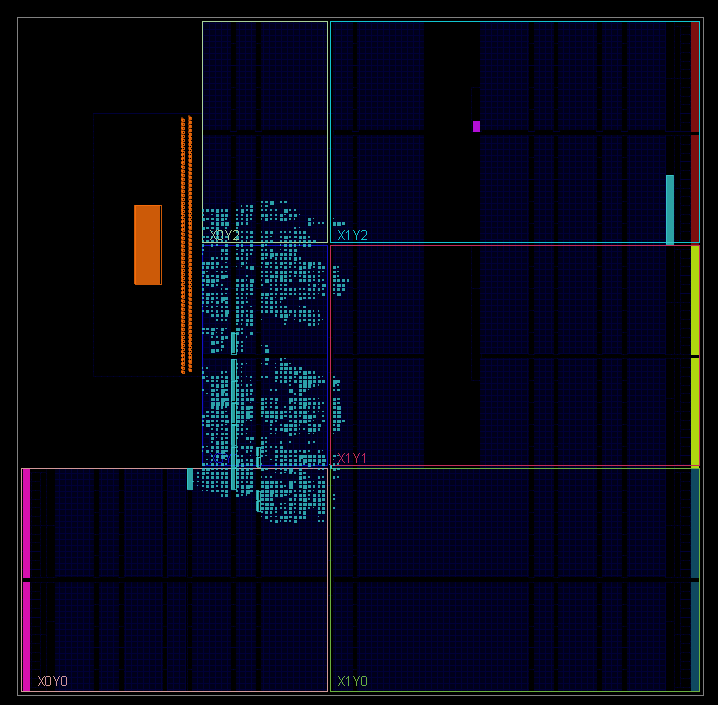
\includegraphics[width=0.28\textwidth]{fig/V0/impl_2.png}
	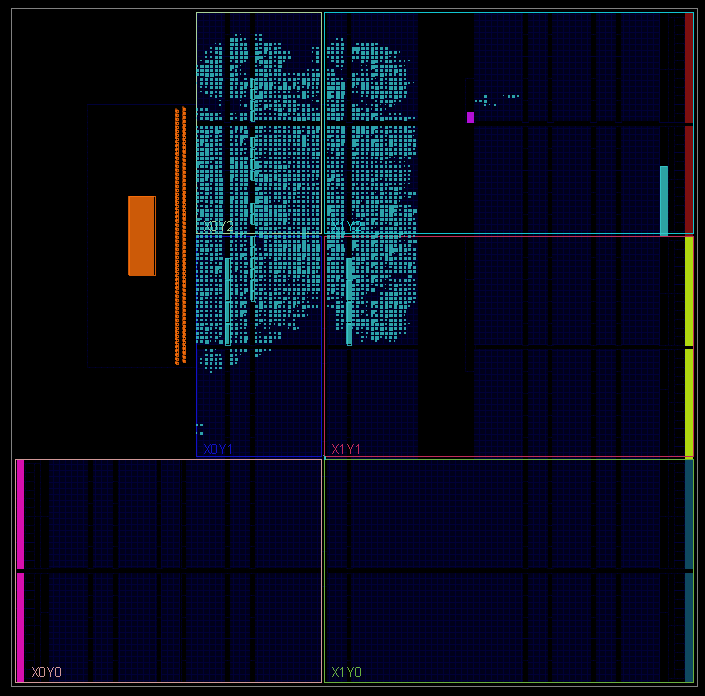
\includegraphics[width=0.28\textwidth]{fig/V0/impl_4.png}
	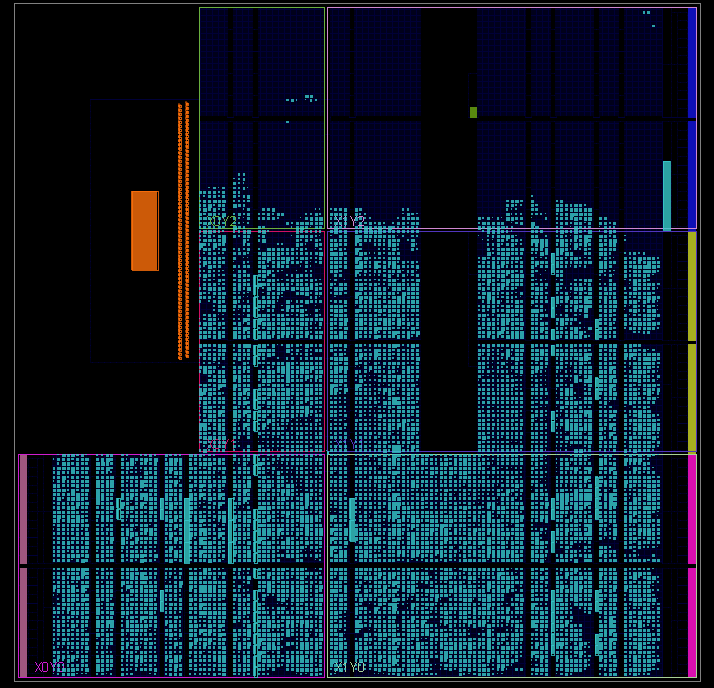
\includegraphics[width=0.28\textwidth]{fig/V0/impl_8.png}
\caption{Implementation Design for V0. 좌측부터 RAM\_SIZE의 크기를 1, 2, 3으로 변화시켜 (행렬 곱셈에 사용되는 행렬의 크기를 2*2, 4*4, 8*8로 바꿔가며) bitstream을 생성한 결과이다. }
\label{impl_v0}
\end{figure}

\subsubsection{Benchmark Result}
\begin{figure}[htb!]
	\centering
	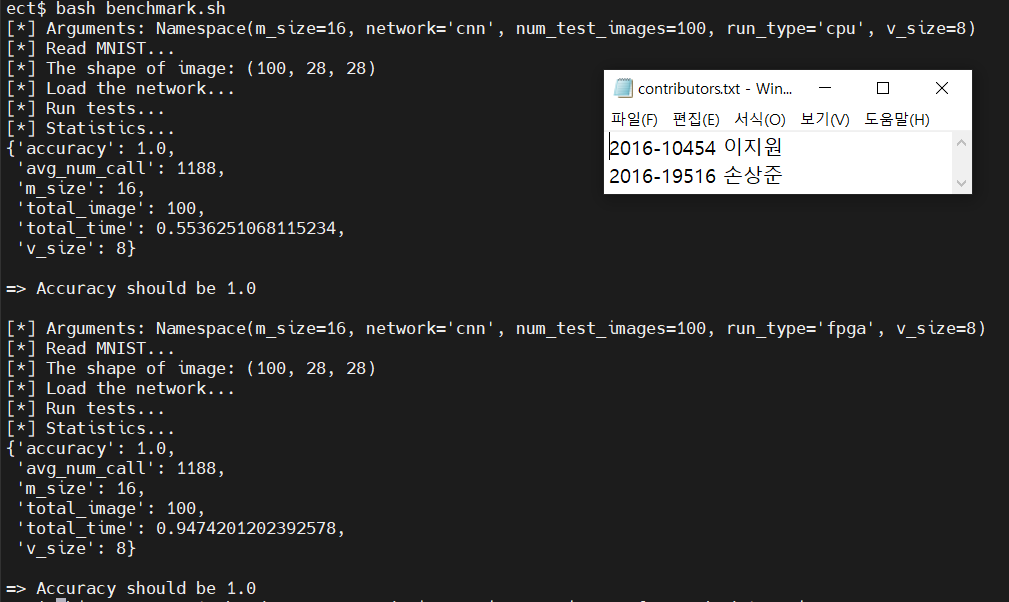
\includegraphics[width=0.6\textwidth]{fig/V0/benchmark.png}
\caption{Benchmark Result for V0. 테스트 이미지 갯수를 100장으로 한 뒤 8*8 행렬 곱셈을 각각 run\_type을 CPU 버전, FPGA 버전으로 실행한 결과이다. CPU를 사용한 결과가 약 2배 정도 빠른 속도를 보인 것으로 보아 FPGA 가속기의 이상적인 성능 향상을 이룩하진 못하였다. }
\label{benchmark_v0}
\end{figure}

\subsection{Optimization: DMA}
\subsubsection{Implementation \& Benchmark Result}
\begin{figure}[htb!]
	\centering
	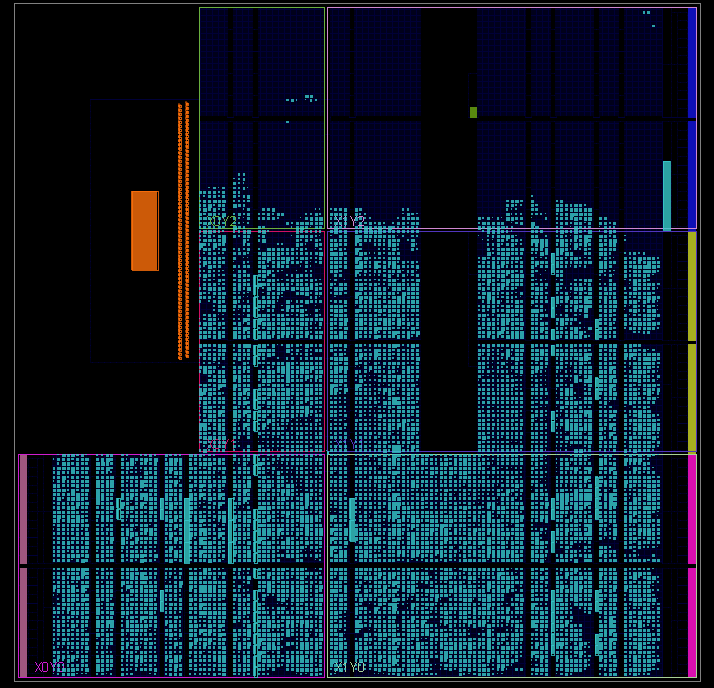
\includegraphics[width=0.37\textwidth]{fig/V1_DMA/impl.png}
	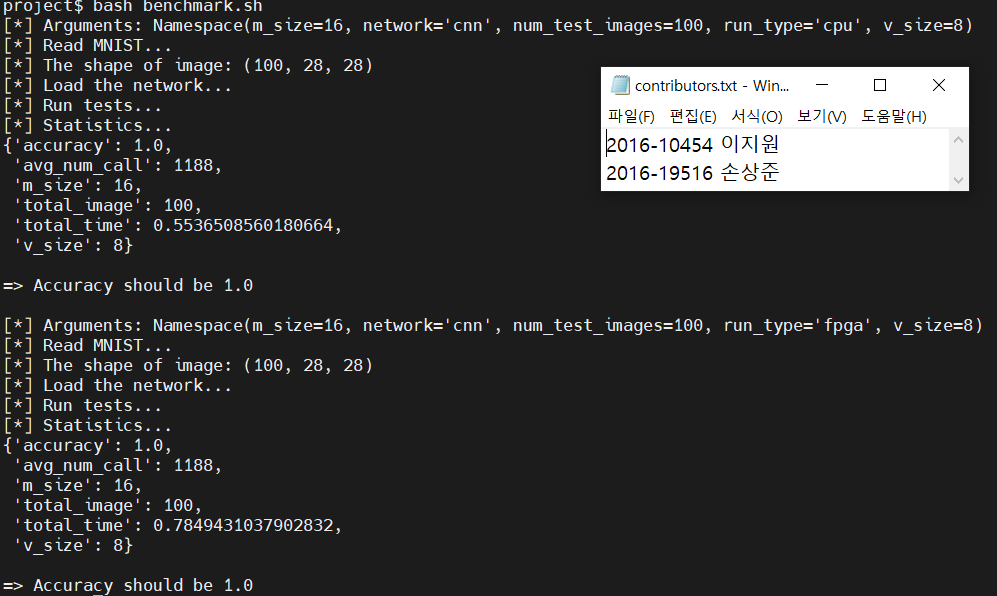
\includegraphics[width=0.60\textwidth]{fig/V1_DMA/benchmark.png}
\caption{Implementation Design \& Benchmark Result for V1\_DMA. 테스트 이미지 갯수를 100장으로 한 뒤 8*8 행렬 곱셈을 각각 run\_type을 CPU 버전, FPGA 버전으로 실행한 결과이다. }
\label{impl_v1_dma}
\end{figure}

\subsection{Optimization: Quantization}

\subsubsection{Implementation}
\begin{figure}[htb!]
	\centering
	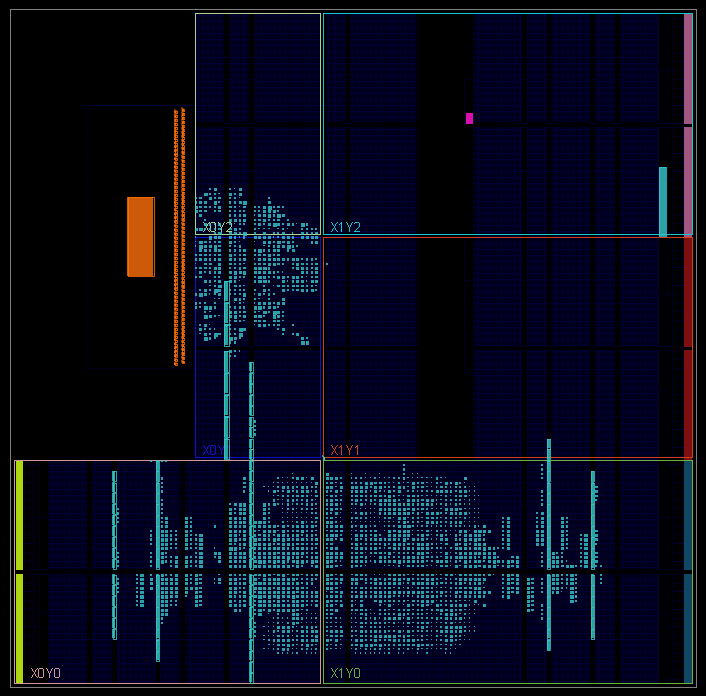
\includegraphics[width=0.4\textwidth]{fig/V1_Quantization/impl.png}
\caption{Implementation Design for V1\_Quantization.}
\label{impl_v1_quantization}
\end{figure}
\subsubsection{Benchmark Result}
\begin{figure}[htb!]
	\centering
	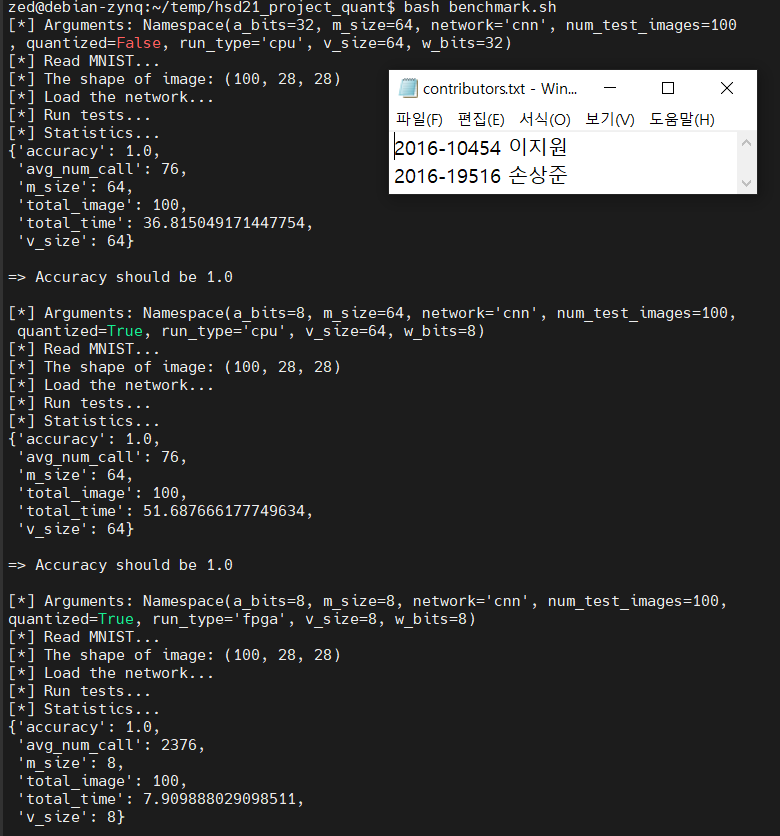
\includegraphics[width=0.60\textwidth]{fig/V1_Quantization/benchmark.png}
\caption{Benchmark Result for V1\_Quantization. 상단부터 테스트 이미지 갯수를 100장으로 한 뒤 64*64 행렬 곱셈을 각각 양자화되지 않은 CPU 버전, 양자화된 CPU 버전과 최하단에는 8*8 FPGA 버전으로 실행한 결과이다. }
\label{benchmark_v1_quantization}
\end{figure}

\section{Conclusion}
지난 번 프로젝트 중간 제출 당시에 simulation 상에서 동작하는 것을 목표로 진행했기 때문에 보드에서 동작하는 것은 확인하지 않았다. Matrix-Matrix Multiplication를 구현하기 위해서는 PE가 여러 개 필요하였고 이를 위해서는 for generate를 사용하여 코드의 반복을 막을 수 있었고 가독성 또한 높일 수 있었다. \\

이번에 FPGA를 구현하기 위해서 Verilog 모듈을 구현하는 것만이 가속기를 만드는 주요 부분이 아니라는 것을 알 수 있었다. BRAM을 연결하거나 소프트웨어 상에서 주소를 잘못 참조하거나 LUT 또는 FF 개수가 너무 많아 state를 여러 개로 쪼개어 구현하는 등 여러가지 이슈가 있어왔으며 보고서에 언급하지 않은 구현 상에 여러가지 문제점이 많이 있었다. \\

프로젝트를 통해 처음으로 Quantization 및 DMA를 구현해 볼 수 있었다. 더 적은 Bit의 연산을 수행하고 더 적은 cycle을 소모하여 정수 곱셈을 수행하였기에 보다 빠른 연산이 가능했다. 정확도가 확연히 떨어질 것으로 예상했으나 그렇지 않았다. DMA의 경우 데이터 전송에서 걸리는 시간을 눈에 띌 정도로 절약하여 결국 행렬 곱셈에 걸리는 시간을 줄일 수 있었다. \\

\section*{Acknowledgments}
하드웨어 실습 설계에서 배운 모든 테크닉들이 차후 유용하게 쓰일 것 같아 아주 뿌듯한 한 학기였습니다. 그동안 함께 고생한 팀원 이지원, 손상준과 열심히 지도해주신 유승주 교수님, 조교분들에게 감사의 인사를 드립니다. \\

\bibliographystyle{plain}
\bibliography{other}

\newpage
\appendix
\section{Testbench for MM-multiplication module}
Matrix 2개의 값들은 input.txt에 저장한다. input.txt에 저장된 값을 읽어들여, output.txt로 결과값을 출력시킨다. 아래의 waveform은 testbench를 통해 얻어진 결과값이다.

\begin{figure}[htb!]
	\centering
	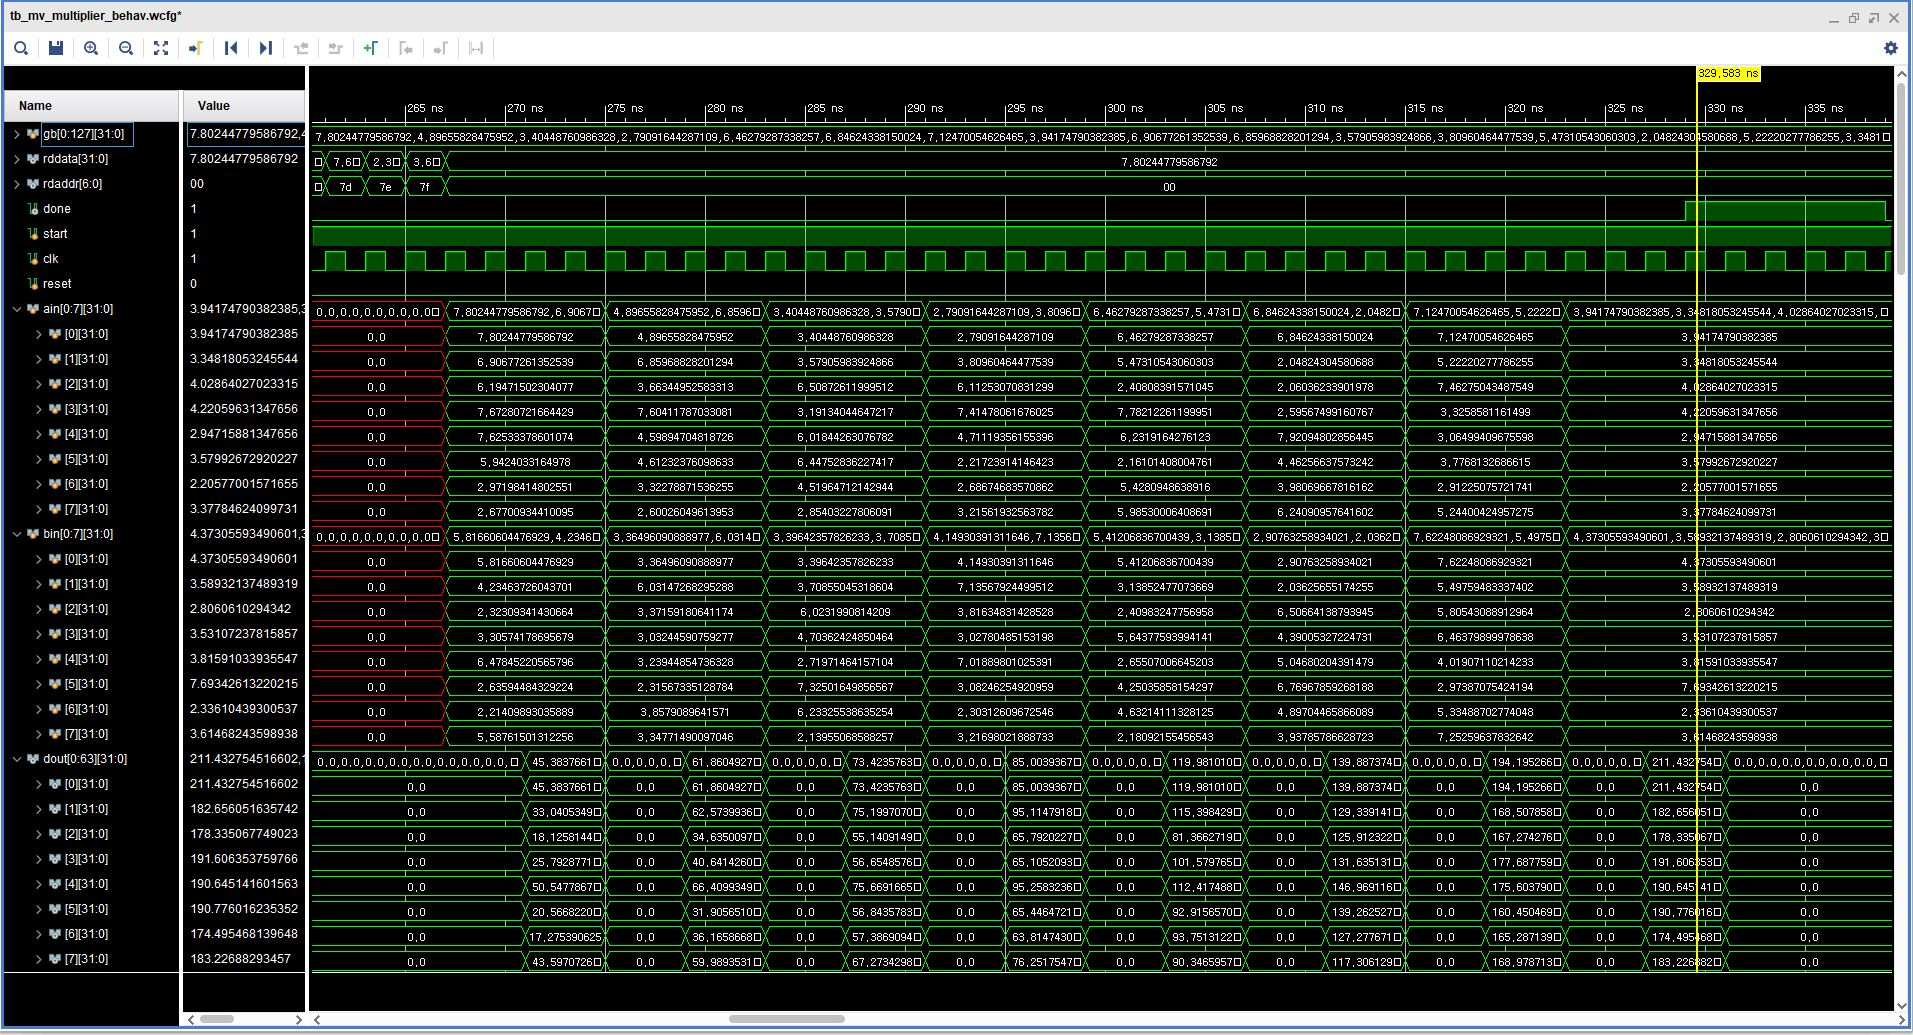
\includegraphics[width=0.8\textwidth]{fig/mm1.jpg}
	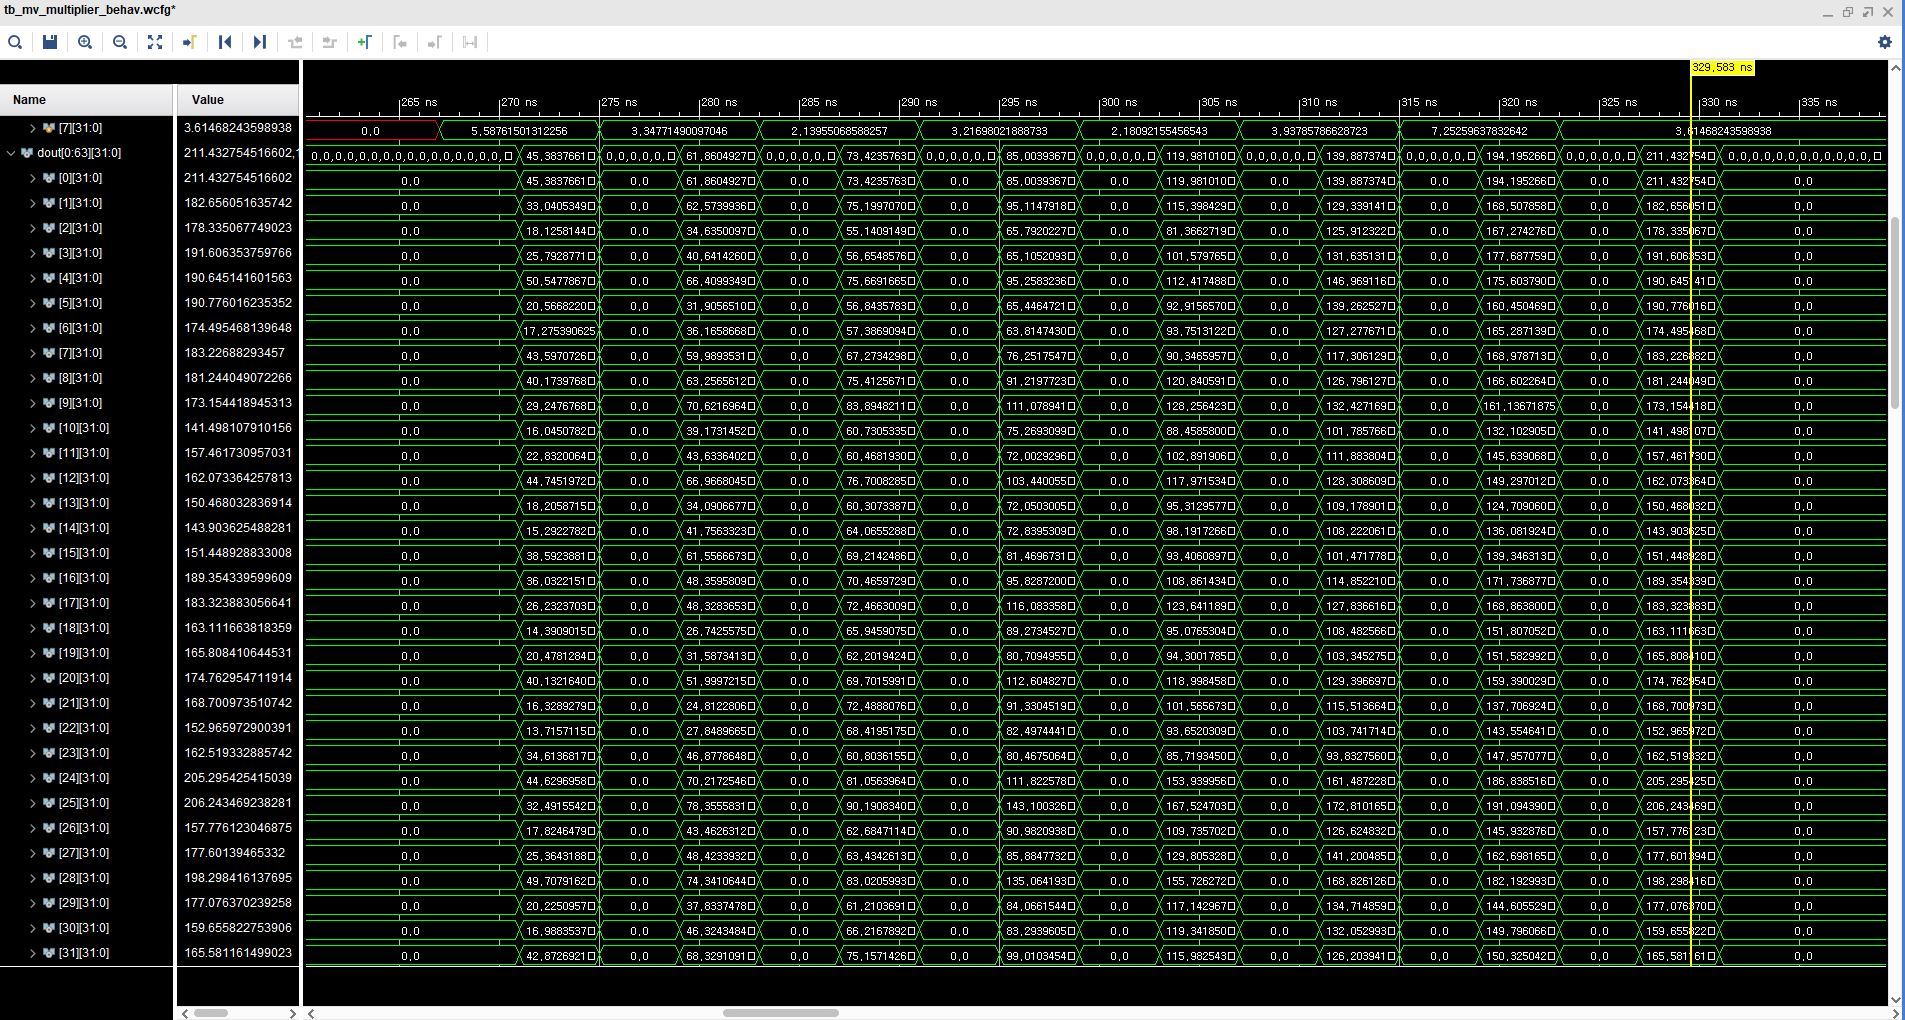
\includegraphics[width=0.8\textwidth]{fig/mm2.jpg}
\caption{Broadcast \& PE computation process}
\label{testbench}
\end{figure}
ain, bin은 PE모듈의 input이고, PE는 내적을 수행하기 때문에, \texttt{ain}은 Matrix-Matrix multiply에서 첫 번째 matrix그대로 들어가고, \texttt{bin}은 두 번째 Matrix의 전치행렬이다.

\section{Floating-point MM multiplication test dataset}
\label{sec:float}
\hfill
\begin{adjustbox}{angle=90}
\resizebox{0.95\textheight}{!}{
\begin{tabular}{|c|rrrrrrrr|c|rrrrrrrr|}
\hline
A & \multicolumn{1}{c}{0} & \multicolumn{1}{c}{1} & \multicolumn{1}{c}{2} & \multicolumn{1}{c}{3} & \multicolumn{1}{c}{4} & \multicolumn{1}{c}{5} & \multicolumn{1}{c}{6} & \multicolumn{1}{c|}{7} & B & \multicolumn{1}{c}{0} & \multicolumn{1}{c}{1} & \multicolumn{1}{c}{2} & \multicolumn{1}{c}{3} & \multicolumn{1}{c}{4} & \multicolumn{1}{c}{5} & \multicolumn{1}{c}{6} & \multicolumn{1}{c|}{7} \\ \hline
0 & 40f9ada7 & 409cb09b & 4059e320 & 40329e60 & 40cecf33 & 40db146d & 40e3fd8c & 407c4599 & 0 & 40ba21a3 & 40878226 & 4014ad90 & 40539146 & 40cf4f7b & 4028b352 & 400db3cc & 40b2cdbe \\
1 & 40dd0448 & 40db8291 & 40650f51 & 4073d090 & 40af23ae & 4003166a & 40a71c49 & 40564897 & 1 & 40575b85 & 40c101d3 & 4057c829 & 40421398 & 404f5320 & 401433fe & 4076e7fb & 405640f6 \\
2 & 40c63b1b & 406a75f5 & 40d0477c & 40c399da & 401a1e0c & 4003dcfa & 40eeceda & 4080ea9f & 2 & 40595f01 & 406d58e4 & 40c0be0c & 40968417 & 402e0fce & 40ea6689 & 40c776d4 & 4008ee66 \\
3 & 40f587a3 & 40f354ef & 404c3eec & 40ed45e2 & 40f90726 & 40261f8a & 4054dadc & 40870f20 & 3 & 4084c719 & 40e4577c & 40743f0d & 4041c78e & 40e09ad0 & 40454711 & 4013666b & 404de301 \\
4 & 40f402bc & 40932a93 & 40c09715 & 4096c219 & 40c76bdc & 40fd7868 & 404428dd & 403c9e40 & 4 & 40ad2faa & 4048dd97 & 401a3ab2 & 40b499d0 & 4029ecab & 408802f0 & 40943a80 & 400b9438 \\
5 & 40be282b & 40939828 & 40ce5227 & 400de73f & 400a4e0e & 408ecd58 & 4071b74f & 40651d85 & 5 & 403a16a7 & 40025207 & 40d03668 & 408c7b51 & 40a17f67 & 40d8a135 & 409cb497 & 407c05dd \\
6 & 403e34fd & 4054a892 & 4090a0f3 & 402bf3a9 & 40adb2f4 & 407ec3bc & 403a6251 & 400d2b56 & 6 & 40f3eb5d & 40afec4c & 40b9c617 & 40ced771 & 40809c3b & 403e53e6 & 40aab765 & 40e81545 \\
7 & 402b541f & 40266aab & 4036a877 & 404dccb5 & 40bf8794 & 40c7b588 & 40a7cee2 & 40582ea2 & 7 & 408bf013 & 4065b771 & 40339681 & 4061fd17 & 407437e0 & 40f6308c & 401582bc & 406756f5 \\ \hline
C & \multicolumn{1}{c}{0} & \multicolumn{1}{c}{1} & \multicolumn{1}{c}{2} & \multicolumn{1}{c}{3} & \multicolumn{1}{c}{4} & \multicolumn{1}{c}{5} & \multicolumn{1}{c}{6} & \multicolumn{1}{c|}{7} &  & \multicolumn{1}{c}{} & \multicolumn{1}{c}{} & \multicolumn{1}{c}{} & \multicolumn{1}{c}{} & \multicolumn{1}{c}{} & \multicolumn{1}{c}{} & \multicolumn{1}{c}{} & \multicolumn{1}{c|}{} \\ \hline
0 & 43536ec9 & 4336a7f3 & 433255c7 & 433f9b3a & 433ea528 & 433ec6a9 & 432e7ed7 & 43373a15 &  &  &  &  &  &  &  &  &  \\
1 & 43353e7a & 432d2788 & 430d7f84 & 431d7634 & 432212c8 & 431677d1 & 430fe754 & 431772ed &  &  &  &  &  &  &  &  &  \\
2 & 433d5ab6 & 433752ea & 43231c96 & 4325cef4 & 432ec351 & 4328b373 & 4318f74a & 432284f3 &  &  &  &  &  &  &  &  &  \\
3 & 434d4ba1 & 434e3e54 & 431dc6b0 & 433199f5 & 43464c65 & 4331138d & 431fa7e4 & 432594c7 &  &  &  &  &  &  &  &  &  \\
4 & 4340d3f1 & 4333152d & 433411f4 & 4335e3bb & 4341d207 & 43494175 & 432de216 & 4323b37a &  &  &  &  &  &  &  &  &  \\
5 & 43164c64 & 430e329f & 430ede1e & 430b82f3 & 430fa2e2 & 431e937f & 43089f44 & 430430b0 &  &  &  &  &  &  &  &  &  \\
6 & 42ff8693 & 42eb4228 & 42eb52cf & 42f8091f & 42e7952b & 43049116 & 42ee2c16 & 42cd4d8f &  &  &  &  &  &  &  &  &  \\
7 & 4318a3d3 & 4304ff07 & 430b66c0 & 4312e57d & 430973c0 & 43192a9f & 43074efe & 42fff8b2 &  &  &  &  &  &  &  &  &  \\ \hline
A & \multicolumn{1}{c}{0} & \multicolumn{1}{c}{1} & \multicolumn{1}{c}{2} & \multicolumn{1}{c}{3} & \multicolumn{1}{c}{4} & \multicolumn{1}{c}{5} & \multicolumn{1}{c}{6} & \multicolumn{1}{c|}{7} & B & \multicolumn{1}{c}{0} & \multicolumn{1}{c}{1} & \multicolumn{1}{c}{2} & \multicolumn{1}{c}{3} & \multicolumn{1}{c}{4} & \multicolumn{1}{c}{5} & \multicolumn{1}{c}{6} & \multicolumn{1}{c|}{7} \\ \hline
0 & 7.8024 & 4.8966 & 3.4045 & 2.7909 & 6.4628 & 6.8462 & 7.1247 & 3.9417 & 0 & 5.8166 & 4.2346 & 2.3231 & 3.3057 & 6.4785 & 2.6359 & 2.2141 & 5.5876 \\
1 & 6.9068 & 6.8597 & 3.5791 & 3.8096 & 5.4731 & 2.0482 & 5.2222 & 3.3482 & 1 & 3.3650 & 6.0315 & 3.3716 & 3.0324 & 3.2394 & 2.3157 & 3.8579 & 3.3477 \\
2 & 6.1947 & 3.6634 & 6.5087 & 6.1125 & 2.4081 & 2.0604 & 7.4628 & 4.0286 & 2 & 3.3964 & 3.7086 & 6.0232 & 4.7036 & 2.7197 & 7.3250 & 6.2333 & 2.1396 \\
3 & 7.6728 & 7.6041 & 3.1913 & 7.4148 & 7.7821 & 2.5957 & 3.3259 & 4.2206 & 3 & 4.1493 & 7.1357 & 3.8163 & 3.0278 & 7.0189 & 3.0825 & 2.3031 & 3.2170 \\
4 & 7.6253 & 4.5989 & 6.0184 & 4.7112 & 6.2319 & 7.9209 & 3.0650 & 2.9472 & 4 & 5.4121 & 3.1385 & 2.4098 & 5.6438 & 2.6551 & 4.2504 & 4.6321 & 2.1809 \\
5 & 5.9424 & 4.6123 & 6.4475 & 2.2172 & 2.1610 & 4.4626 & 3.7768 & 3.5799 & 5 & 2.9076 & 2.0363 & 6.5066 & 4.3901 & 5.0468 & 6.7697 & 4.8970 & 3.9379 \\
6 & 2.9720 & 3.3228 & 4.5196 & 2.6867 & 5.4281 & 3.9807 & 2.9123 & 2.2058 & 6 & 7.6225 & 5.4976 & 5.8054 & 6.4638 & 4.0191 & 2.9739 & 5.3349 & 7.2526 \\
7 & 2.6770 & 2.6003 & 2.8540 & 3.2156 & 5.9853 & 6.2409 & 5.2440 & 3.3778 & 7 & 4.3731 & 3.5893 & 2.8061 & 3.5311 & 3.8159 & 7.6934 & 2.3361 & 3.6147 \\ \hline
C & \multicolumn{1}{c}{0} & \multicolumn{1}{c}{1} & \multicolumn{1}{c}{2} & \multicolumn{1}{c}{3} & \multicolumn{1}{c}{4} & \multicolumn{1}{c}{5} & \multicolumn{1}{c}{6} & \multicolumn{1}{c|}{7} &  & \multicolumn{1}{c}{} & \multicolumn{1}{c}{} & \multicolumn{1}{c}{} & \multicolumn{1}{c}{} & \multicolumn{1}{c}{} & \multicolumn{1}{c}{} & \multicolumn{1}{c}{} & \multicolumn{1}{c|}{} \\ \hline
0 & 211.4328 & 182.6561 & 178.3351 & 191.6064 & 190.6451 & 190.7760 & 174.4955 & 183.2269 &  &  &  &  &  &  &  &  &  \\
1 & 181.2440 & 173.1544 & 141.4981 & 157.4617 & 162.0734 & 150.4680 & 143.9036 & 151.4489 &  &  &  &  &  &  &  &  &  \\
2 & 189.3543 & 183.3239 & 163.1117 & 165.8084 & 174.7630 & 168.7010 & 152.9660 & 162.5193 &  &  &  &  &  &  &  &  &  \\
3 & 205.2954 & 206.2435 & 157.7761 & 177.6014 & 198.2984 & 177.0764 & 159.6558 & 165.5812 &  &  &  &  &  &  &  &  &  \\
4 & 192.8279 & 179.0827 & 180.0701 & 181.8896 & 193.8204 & 201.2557 & 173.8831 & 163.7011 &  &  &  &  &  &  &  &  &  \\
5 & 150.2984 & 142.1977 & 142.8676 & 139.5115 & 143.6363 & 158.5762 & 136.6221 & 132.1902 &  &  &  &  &  &  &  &  &  \\
6 & 127.7628 & 117.6292 & 117.6617 & 124.0178 & 115.7913 & 132.5667 & 119.0861 & 102.6515 &  &  &  &  &  &  &  &  &  \\
7 & 152.6399 & 132.9962 & 139.4014 & 146.8964 & 137.4521 & 153.1665 & 135.3086 & 127.9857 &  &  &  &  &  &  &  &  &  \\ \hline
\end{tabular} \newline
}\end{adjustbox}
\hfill
\null

\end{document}
